\chapter{Wind Turbine qLPV Models} \label{sec:WindTurbineqLPVModels}
A wind turbine is a highly complex mechanical system. However, control-oriented models only aim to represent the dynamics that either provide information to the controller or are influenced by the actuator settings commanded by the controller. Therefore, the resulting models are of relatively low order. In Section  \ref{sec:MechanicalAerodynamicSubsystemModel}, the physical equations that serve as the basis for building a Simulink model of the turbine dynamics, and for the underlying models for the qLMPC algorithm discussed in the next chapter, are presented. The two first-principle models derived in this chapter are compared in Section \ref{sec:qLPVModelVerificationwithFAST0} in the time and frequency domains against the wind turbine simulation code FAST. The presented models have been published in \cite{dittmer2021velocity}.

\section{Nonlinear Models for qLMPC Design} \label{sec:MechanicalAerodynamicSubsystemModel}
Figure~\ref{fig:SchWTDefl} illustrates the movements and deflections of the tower and blades as a result of the forces and moments acting on them.
These structural deflections are associated with specific turbine modes, which represent distinct oscillations occurring at characteristic frequencies. Controllers are designed to dampen these modes to prevent excessive oscillations which may lead to fatigue loading and, in severe cases, dynamic instability and structural failure. If not properly controlled, these oscillations may resonate with the turbine’s natural frequencies, potentially causing harm to components or reducing its operational lifespan. Therefore, a mathematical model of the turbine must account for these modes to ensure accurate control and safe operation. 

Figure~\ref{fig:SchWTLPV} depicts the inputs, states, and geometric parameters utilized in the qLPV model of the wind turbine. Following the NREL 5MW documentation \cite{jonkman2009definition}, the tower-base coordinate system is defined with the x-axis pointing downwind, the y-axis transverse to the wind direction, and the z-axis vertical from tower base to yaw bearing. 
The blade coordinate system is defined according to the FAST documentation \cite{jonkman2005fast}: For each blade \(i = 1, 2, 3\), the axis definitions are as follows: the \(x_{bi}\)-axis is orthogonal to the \(y_{bi}\)- and \(z_{bi}\)-axes such that the three form a right-handed coordinate system, the \(y_{bi}\)-axis points toward the trailing edge of blade \(i\) and is parallel to the chord line at the zero-twist blade station, and the \(z_{bi}\)-axis points along the pitch axis toward the tip of blade \(i\). Consequently, the \(x_{bi}\)-axis denotes flapwise blade motion, the \(y_{bi}\)-axis edgewise motion, and torsion of the blade is defined as the rotation about the \(z_{bi}\)-axis. 

The geometric parameters depicted are the hub height $H_t$ and the rotor radius $R_r$. The model inputs are the rotor and generator torques, $T_r$ and $T_g$, as well as the rotor thrust $F_{T,r}$, which results from the wind acting on the wind turbine, $V_r$, which is perpendicular to its rotor. 
\begin{figure}[H]
    \centering
    \begin{minipage}[b]{11.5pc}
        \adjustbox{valign=b}{\includegraphics[width=11.5pc]{figuresBlockDiagram_IFAC23/windTurbineModesTwrBld01.pdf}}
        \caption{\label{fig:SchWTDefl}Schematic wind turbine diagram of tower and blade movements.}
    \end{minipage}
    \hspace{3pc}
    \begin{minipage}[b]{13.7pc}
        \adjustbox{valign=b}{\includegraphics[width=13.7pc]{figuresBlockDiagram_IFAC23/wind turbine 01.pdf}}
        \caption{\label{fig:SchWTLPV}Schematic LPV wind turbine model diagram with inputs, states, and parameters.}
    \end{minipage}
\end{figure}
%\noindent
Two qLPV designs are introduced in this section: the first models the rotor speed and the tower movement, while the second additionally accounts for the generator speed and the blade deflection. Both models use the three inputs rotor torque, generator torque, and thrust force.

The five states of the first model considered are the fore-aft and side-to-side tower deflections at hub height, $x_t$ and $y_t$, as well as their derivatives, $\dot{x}_t$ and $\dot{y}_t$, i.e., the fore-aft and side-to-side velocities, and the angular rotor speed $\omega_r$.
The state vector of the second model additionally contains the angular generator speed $\omega_g$ and the angular flapwise blade deflection $\delta_b$. Note that both the wind speed and the resulting force act in a distributed manner over the rotor disk. The vectors $V_r$ and $F_{T,r}$ give an equivalent one dimensional wind and force vector of the two dimensional wind field distributed over the rotor disk area and the forces acting at the segments of the blades.

 The thrust $F_{T,r}$ is the sum of the accumulated forces acting on the blades of the turbines, with the accumulated force per blade denoted $F_{T,bi}$ for the $i$th blade and with $n_b$ as the number of blades. To model the hub's movement and the resulting mechanical moments from the thrust force $F_{T,r}$, these forces are consolidated into a single force acting at a specific point on the blade, which is located at a distance $r_b$ from the rotor hub. This uses the same modeling as in \cite{Bianchi2007} where "the thrust forces distributed along each blade were
 replaced by a lumped force $F_T$ applied at a distance $r_b$ from the axis of rotation". 
In the following subsections, the underlying equations for two qLPV models are provided. Both turbine models share the drivetrain and actuator models, as well as the same aerodynamics model. The servo-elastic modeling of the first model is based on two simple physical equations governing the rotational motion and the tower bending. The more advanced servo-elastic modeling of the second model is derived from Lagrange's equation.

\subsection{Drivetrain, Torque Actuator, and Pitch Actuator Models}\label{subsec:drivetrain, Torque Actuator, and Pitch Actuator Models}
The flexible drivetrain subsystem, which contains a high-speed and a low-speed shaft, as well as a gearbox, transmits the aerodynamic torque to the generator. Linking multiple rigid bodies with flexible joints via a drivetrain results in a highly non-linear system, i.e., a system with dynamics that depend heavily on the operating point. However, for a control-oriented model, a system with one or two degrees of freedom in the rotational plane suffices, see, e.g., \cite{Bianchi2007}, \cite{peeters2006analysis} or  \cite{sharan2018actuator}.  
%
The drivetrain is modeled as a two-mass system, with the gearbox as a rigid body and the drivetrain's flexibility represented by a torsion spring on the low-speed shaft. The drivetrain dynamics are given by the following continuous first-order differential equations  \cite{sharan2018actuator}:
\begin{align} 
    J_{r}\dot{\omega_{r}}(t) &= T_{r}(t) - T_{\text{lss}}(t), \quad T_{\text{lss}}(t) = K_{s}\theta_{s}(t), \quad T_{\text{lss}}(t) = N_{g}T_{\text{hss}}(t), \nonumber\\
    J_{g}\dot{\omega_{g}}(t) &= \frac{1}{N_{g}} T_{\text{lss}}(t) - T_{g}(t), \quad \dot{\theta}_{s}(t) = \omega_{r}(t) - \frac{1}{N_{g}} \omega_{g}(t), \label{eq:DrvTr}
\end{align}
with angular rotor and generator speeds $\omega_{r}$ and $\omega_{g}$ and their respective torques $T_{r}$ and $T_{g}$. The low-speed and high-speed shaft torques are denoted by $T_{\text{lss}}$ and $T_{\text{hss}}$, while $J_{r}$ and $J_{g}$ represent the combined inertia on the rotor and generator sides, respectively. The torsion stiffness of the drivetrain is indicated by $K_{s}$, the gear ratio is given as $N_{g}$, and $\theta_{s}$ denotes the drivetrain's torsion angle. The torsional flexibility is neglected as the torsional mode lies above the frequency range of interest for power control. This allows the simplification $\dot{\omega}_g = N_g \dot{\omega}_r$ which results in
\begin{align} \label{eq:DrivetrainStiff}
     J_{g}N_g \dot{\omega}_r(t) = \frac{1}{N_{g}} T_{\text{lss}}(t) - T_{g}(t) \iff J_{g}N^2_g \dot{\omega}_r(t) = T_{\text{lss}}(t) - N_gT_{g}(t).
\end{align}
Combining Equation \eqref{eq:DrivetrainStiff} with the first equation from the Equations \eqref{eq:DrvTr} allows representing the rotor speed rate as
\begin{align*}
    \underbrace{(J_r + N^2_g J_g)}_{J_s}\dot{\omega}_r(t)= T_r(t) - N_g T_g(t)
\end{align*}
with the transmission inertia $J_s$. The extracted power $P_{g}$ is the product of the generator efficiency $\eta_{g}$ and the power $P_r$, i.e., the power extracted by the rotor from the available wind power $P_w$. It can be calculated as 
\begin{align}\label{eq:pg}
    P_{g}(t) = \eta_{g} T_{g}(t) \omega_{g}(t),
\end{align}
since equations \eqref{eq:DrvTr} show that the product of the rotor's angular speed and torque equals that of the generator in steady-state. Therefore, setting the torque of the generator directly influences the power output of the turbine.
%\noindent
%
The torque actuator can be regarded as the power conditioning unit of the turbine, and its dynamics can be modeled as a first-order differential equation \cite{odgaard2013fault}:
\begin{align}\label{eq:Tact}
    \dot{T}_{g}(t) = -\frac{1}{\kappa} T_{g}(t) + \frac{1}{\kappa} T_{g,\text{ref}}(t), 
\end{align}
where $\kappa$ denotes the torque actuator model parameter, and $T_{g,\text{ref}}$ is the reference generator torque.

Similarly, a first-order model with time constant $\tau$ is used in this work for the collective pitch $\beta_0$ of the three turbine blades:
\begin{align}\label{eq:betaact}
    \dot{\beta_0}(t) = -\frac{1}{\tau}\beta_0(t) + \frac{1}{\tau}\beta_{0,\text{ref}}(t).
\end{align}
Although the pitch system is often modeled as a second-order differential equation with natural frequency $\omega_{n,\beta}$ and damping ratio $\zeta_{\beta}$:
\begin{align*}
    \ddot{\beta_0}(t) = -2\zeta_{\beta_0} \omega_{n,\beta} \dot{\beta}_0(t) - {\omega_{n,\beta}}^2 \beta_0(t) + {\omega_{n,\beta}}^2 \beta_{0,\text{ref}}(t),
\end{align*}
the simplified representation as a first order system is made here since the relatively fast actuator dynamics have little influence on the investigated control objectives, which are consistent power output despite wind fluctuations and minimal tower movement. Note that the actuator dynamics, as provided in equations~\eqref{eq:Tact} and \eqref{eq:betaact}, result in low pass filtered signals of the commanded control output signals being applied to the turbine. However, the turbine dynamics, as modeled here in the aerodynamic and mechanical subsystem sections below, operate at much lower frequency and have greater impact on the power output as presented in equation~\eqref{eq:pg}.
\subsection{Aerodynamic Model}
The aerodynamic model represents the conversion of the available kinetic energy in the wind into mechanical energy using the rotor blades. Based on blade actuator disc theory, the mathematical equations for the rotor torque $T_{r}$, the aerodynamic power captured by the rotor $P_{r}$, and the thrust force $F_{T,r}$ can be derived from equations~\eqref{eq:PwPt} and~\eqref{eq:Ft}, used in Section~\ref{sec:WindTurbines} to provide the relationship between wind speed, thrust force and power, as
\begin{equation}\label{eq:aero}
    \begin{split}
        P_{r}(t) & = c_P(\lambda,\beta_0) P_{w}(t) = \frac{1}{2} \rho_a A_r c_P(\lambda,\beta_0) V_r(t)^3, \\
        T_{r}(t) & = \frac{P_{r}(t)}{\omega_{r}(t)} %= \frac{1}{2\omega_{r}(t)} \rho_a A_r c_P(\lambda,\beta_0) V_r(t)^3 \\
        = \frac{R_r}{2\lambda(t)} \rho_a A_r  c_P(\lambda,\beta_0) V_r(t)^{2} \\
        & =  \frac{1}{2} \rho_a R_r A_r  c_Q(\lambda,\beta_0) V_r(t)^{2} ,\\
        F_{T,r}(t) & = \frac{1}{2} \rho_a A_r  c_{T}(\lambda,\beta_0) V_r(t)^{2},
    \end{split}
\end{equation}
where the power, torque, and thrust coefficients $c_P$, $c_Q = c_P/\lambda$, and $c_{T}$ are functions of the blade pitch angle $\beta_0$ and the blade tip speed ratio $\lambda$, which is defined as
\begin{align*}
    \lambda(t) = \frac{\omega_{r}(t) R_r}{V_r(t)}
\end{align*}
and hence depends on the rotor radius $R_r$, the rotor angular speed $\omega_{r}$, and the effective wind speed $V_r$. The 2D matrices for the lookup tables of the power, torque and thrust coefficients, shown in Figure \ref{fig:CPCT}, are generated with the FASTTool.  Alternatively, they could be derived using steady-state FAST simulations with linear, equidistant sweeps of different wind speeds, rotor speeds, and pitch angles, where all input signals are kept constant. This has the advantage that the lookup tables can be designed for the exact version of FAST that is to be used in later calculations. However, as the simulations for the derivation and verification of the qLPV model in this thesis are exclusively done with FAST v8, the lookup tables are derived using functions available in the FASTTool.
%
\begin{figure} [h]
\centering
\subfloat[Power coefficient $c_P$]{%
    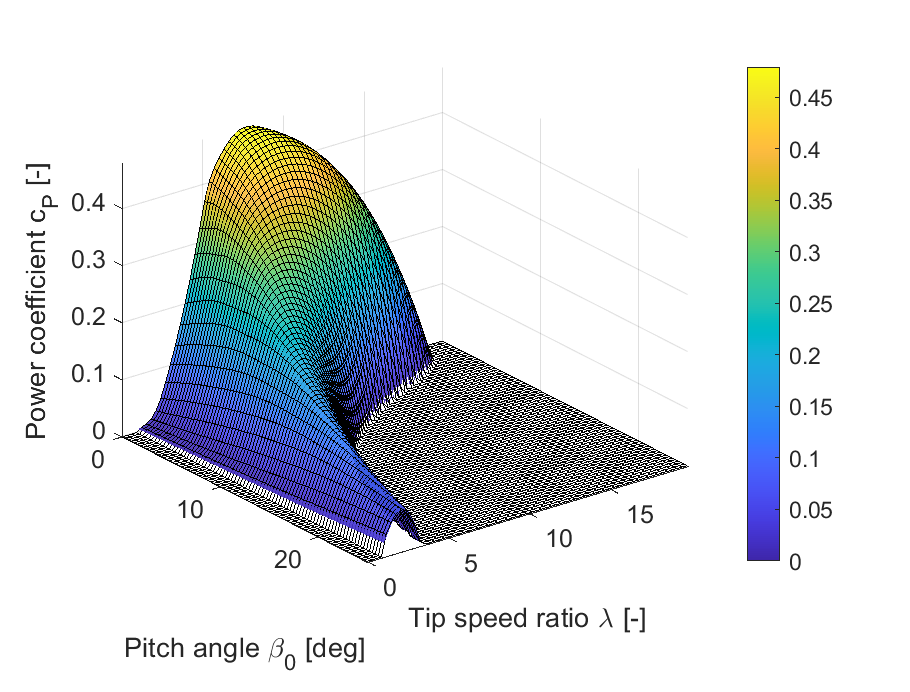
\includegraphics[width=0.49\textwidth]{figures/figDirECC21/Cp_NRRLFAST5MW.eps}
}\hfill
\subfloat[Torque coefficient $c_Q$]{%
    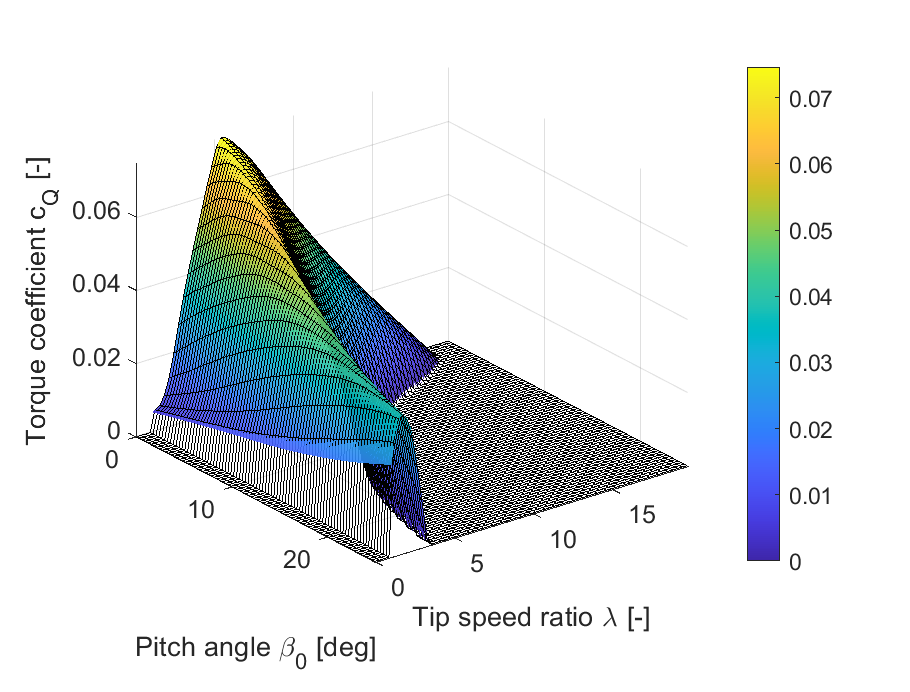
\includegraphics[width=0.49\textwidth]{figures/figDirECC21/Cq_NRRLFAST5MW.eps}
}\\[1ex]
\subfloat[Thrust coefficient $c_T$]{%
    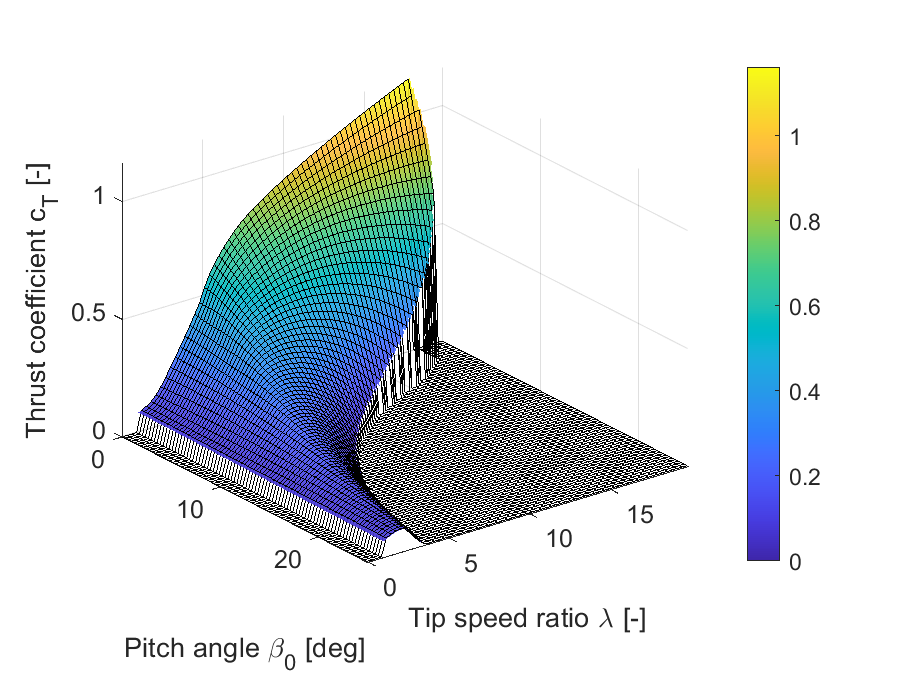
\includegraphics[width=0.49\textwidth]{figures/figDirECC21/Ct_NRRLFAST5MW.eps}
}
\caption{Lookup tables of power, torque and thrust coefficients with respect to blade pitch angle and tip speed ratio for the NREL 5MW model.}
\label{fig:CPCT}
\end{figure}
%
\subsection{Structural Models} \label{subsec:Structural Models}
In this section, two modeling approaches are presented. They are based on previous studies, \cite{schlipf2013nonlinear, mulders2020preventing, Bianchi2007} aiming to derive a structural model and are modified and extended to be amenable for comparison and systematic verification with FAST. Both models leverage the aerodynamic model from Equation~\eqref{eq:aero}. The resulting non-linear differential equations were implemented in Simulink, parameterized using the NREL 5MW turbine parameters given in Table \ref{table:1}, and compared in closed-loop simulations with FAST simulations.
%
\subsubsection{Model 1: Structural Model with Tower Fore–Aft and Side–to–Side Motion}

Models for controller design only need to capture the main dynamics of a system. Hence, the first model uses only the rotor speed, tower displacements and velocities as states. Based on the equations given above, the relationship between the forces and moments acting on the turbine, the inputs, and the rotor speed and tower movements, the states, can be expressed as
\begin{equation}\label{eq:Mdl1NonLin}
    \begin{split} 
        \dot{\omega_r}(t) &= \frac{1}{J_r + N_g^2 J_g}(T_r(t) - N_{g}T_{g}(t)) = \frac{1}{J_s}(T_r(t) - N_{g}T_{g}(t)),   \\
        \ddot{x}_{t}(t) & = \frac{1}{m_{t}}(-B_{t}\dot{x}_{t}(t) - K_{t}{x}_{t}(t) + F_{T,r}(t)), \\
        \ddot{y}_{t}(t) &= \frac{1}{m_{t}}(-B_{t,\text{sw}} \dot{y}_{t}(t) - K_{t,\text{sw}}{y}_{t}(t)  + \frac{3}{2H_t}(T_r(t) - N_gT_g(t))),       
    \end{split}
\end{equation}
where $\omega_r$ is the rotor speed and $x_t$ and $y_t$ represent the fore-aft and side-to-side tower displacements, respectively. The transmission inertia $J_s$ is the combined inertia of the rotor and the generator, see equation \ref{eq:Tr1_background}. The values for the modal tower mass $m_{t}$, fore-aft and side-to-side damping and stiffness terms  $B_t$, $B_{t,\text{sw}}$, $K_t$ and $K_{t,\text{sw}}$, and hub height $H_t$ are provided in Table \ref{table:1}. The values in this table are taken from the documentation of the NREL 5MW research turbine \cite{jonkman2009definition}. 
The calculation of the side-to-side force as
\begin{equation}
    F_{T,y} = \frac{3}{2H_t}(T_r(t) - N_gT_g(t))
\end{equation}
follows from a lumped-force excitation analogous to the fore-aft force in \cite{Bianchi2007}, extended here to the in-plane direction. The reasoning is as follows: the net in-plane torque $\Delta T = T_r - N_g T_g$ acts as a moment at hub height $H_t$. The tower can be regarded as a cantilever beam fixed at the base, with its free end located at hub height. Since the qLPV model captures the tower as a single-degree-of-freedom system represented by the hub-height displacement $y_t$, the equivalent lumped force $F_{T,y}$ is obtained by requiring it to produce the same tip deflection as the applied moment. For a cantilever of length $H_t$, a tip moment $\Delta T$ produces a tip deflection of $\Delta T H_t^2/(2EI)$, while a tip point force $F_{T,y}$ produces a tip deflection of $F_{T,y} H_t^3/(3EI)$,  where $E$ is the modulus of elasticity of the tower material and $I$ is the second moment of area of the tower cross-section. Equating the two gives $F_{T,y}\cdot\tfrac{2}{3}H_t = \Delta T$, which yields the expression above. 
%
While the fore-aft lumped-force model is established in the literature \cite{Bianchi2007} and adopted with minor variations in \cite{mulders2020preventing}, the side-to-side counterpart presented here is, to the author's knowledge, original. The validity of this simplified assumption is confirmed against linearized FAST models in Section~\ref{subsec:ResultsqLPVModel}, where the side-to-side tower response is shown to capture the FAST reference reasonably well around the frequency of the first tower mode, see Figures~\ref{fig:Bode4} and~\ref{fig:Bode12}. 
%
The tower modal mass \( m_t \) is calculated from the total tower weight \( m_{\text{tower}} \), the total nacelle weight \( m_{\text{nacelle}} \), the total hub weight \( m_{\text{hub}} \), and the total blade weight \( m_{\text{blade}} \) as  
\begin{align} \label{eq:modalMass}
    m_t = \frac{1}{4}m_{\text{tower}} + m_{\text{nacelle}} + m_{\text{hub}} + n_b m_{\text{blade}}.
\end{align} 
This is the same calculation of the modal mass as suggested in \cite{schlipf2013nonlinear}.
The damping and stiffness fore-aft $K_t$ and $B_t$ and side-to-side terms $K_{t,\text{sw}}$ and $B_{t,\text{sw}}$ are calculated from the corresponding eigenfrequencies $f_{t,\text{fa}}$ and  $f_{t,\text{sw}}$ and damping $\zeta_t$  with the fore-aft terms as
\begin{align} \label{eq:DampingStiffness}
   K_t = (2\pi f_{t,\text{fa}})^2 m_t\quad\text{and}\quad B_t = 2 \zeta_t (2\pi f_{t,\text{fa}}) m_t,
\end{align}
and the side-to-side terms $B_{t,\text{sw}}$ and $K_{t,\text{sw}}$ derived identically based on $f_{t,\text{sw}}$.
 The table also includes the gearbox ratio $N_g$ and the rotor inertia $J_r$, which consists of the hub inertia and the combined blade inertia of all blades. It is assumed that both $F_{T,r}$ and $T_r$ represent the force and torque acting at the nacelle, implicitly accounting for the forces from all three blades. %The force acting on the rotor in the side-to-side direction is 
% \begin{align*} F_{y_t} = \frac{3}{2H_t}(T_r - N_gT_g).\end{align*}
%    
The vectors for the inputs and states of the linear first and second-order differential equations from the equation set \eqref{eq:Mdl1NonLin} are defined as:
\begin{equation}\label{eq:NonLinInputDef}
    \begin{split}
        \bm{w} &= [F_{T,r} \quad T_r \quad T_g ]^T  \in \mathbb{R}^{3 \times 1},\\
        \bm{x}_{\text{Mdl1}} &= [ x_{t} \quad y_{t} \quad \dot{x}_{t} \quad \dot{y}_{t} \quad \omega_r]^T \in \mathbb{R}^{5 \times 1}.
    \end{split}
\end{equation}
The control inputs of the model are the reference torque and pitch, with the wind acting as a disturbance. This model does not include the dynamics between the reference generator torque and blade pitch, $T_{g,\text{ref}}$ and $\beta_{0,\text{ref}}$, and the actual inputs $T_{g}$ and $\beta_{0}$. Therefore, the first-order actuator dynamics from equations \eqref{eq:Tact} and \eqref{eq:betaact} need to be concatenated with the turbine dynamics in the simulation. Thus, the turbine inputs are the actuator outputs and the wind 
\begin{align} \label{eq:CtrlInputDef}
    \bm{w}_{\text{Mdl}} &= [ V_{\infty} \quad T_{g} \quad \beta_{0}]^T \in \mathbb{R}^{3 \times 1},
\end{align}
where the freestream wind $V_{\infty}$ and the effective wind speed $V_r$ differ by the tower movement, i.e., $V_r = V_{\infty} - \dot{x}_t$.
The gradients of the aerodynamic thrust and torque at an operating point need to be calculated to derive a model using the real inputs provided in the vector $\bm{w}_{\text{Mdl}}$ instead of the fictitious ones in vector $\bm{w}$. The variations of thrust and torque around an operating point depend on changes in the effective wind speed $V_r$, and hence in the disturbance input $V_{\infty}$ and the state $\dot{x}_t$, as well as on changes in the state $\omega_r$ and the control input $\beta_{0}$:
\begin{equation} \label{eq:FTTRGrad}
    \begin{split}
        \hat{F}_{T,r}(t) &= k_{F_T,V} \left( \hat{V}_{\infty}(t) - \hat{\dot{x}}_{t}(t)\right) + \; B_{F_T} \hat{\omega_r}(t) +  k_{F_T,\beta} \hat{\beta_0}(t), \\
        \hat{T}_r(t) &= k_{T_r,V} \left( \hat{V}_{\infty}(t) - \hat{\dot{x}}_{t}(t)\right) + B_{T_r} \hat{\omega_r}(t) + k_{T_r,\beta} \hat{\beta_0}(t),
    \end{split}
\end{equation} \enlargethispage{\baselineskip}
with a hat denoting a variation with respect to a steady-state. Substituting the terms from equations \eqref{eq:FTTRGrad} into equations \eqref{eq:Mdl1NonLin} yields a linear model describing the influence of changes in the inputs $\bm{w}_{\text{Mdl}}$ on the states $x_{\text{Mdl1}}$ from equations \eqref{eq:NonLinInputDef} and~\eqref{eq:CtrlInputDef}. The partial derivatives of the rotor thrust force and torque are calculated from the equation set~\eqref{eq:aero} with $[F_{T_r} \quad T_r] = [k_{c_T} c_T(\lambda,\beta_0) V_r^2 \quad k_{c_Q}  c_Q(\lambda,\beta_0) V_r^2]$ where the constants are $k_{c_T} = 0.5 \rho_a A_r$ and $k_{c_Q} = 0.5 \rho_a R_r A_r$, respectively. This results in the derivatives: 
\begin{align*}
     k_{F_T,V} = \frac{\partial F_{T,r}(t)}{\partial{V_{\infty}(t)}} \bigg|_{\bar{V}_{\infty},\bar{\omega}_r,\bar{\beta}_0} &= k_{c_T}  \bar{V}_{\infty} \left(2\bar{c}_T + \frac{\partial  c_T(\lambda,\beta_0)}{\partial{\lambda(t)}}\bigg|_{\bar{V}_{\infty},\bar{\omega}_r,\bar{\beta}_0}  \frac{ \partial \lambda(t)}{ \partial V_{\infty}(t)}\bigg|_{\bar{V}_{\infty},\bar{\omega}_r,\bar{\beta}_0} \bar{V}_{\infty} \right),\\
    %
    B_{F_T} = \frac{\partial F_{T,r}(t)}{\partial{\omega_r(t) }}  \bigg|_{\bar{V}_{\infty},\bar{\omega}_r,\bar{\beta}_0} &= 
    k_{c_T} \frac{\partial c_{T}(\lambda,\beta_0)}{\partial \lambda(t)} \bigg|_{\bar{V}_{\infty},\bar{\omega}_r,\bar{\beta}_0} \frac{ \partial \lambda(t)}{ \partial \omega_r(t)}\bigg|_{\bar{V}_{\infty},\bar{\omega}_r,\bar{\beta}_0} \bar{V}_{\infty}^2, \\
    %
   k_{F_T,\beta} = \frac{\partial F_{T,r}(t)}{\partial{\beta_0(t) }}  \bigg|_{\bar{V}_{\infty},\bar{\omega}_r,\bar{\beta}_0} &= 
k_{c_T} \frac{\partial c_{T}(\lambda,\beta_0)}{\partial \beta_0(t)} \bigg|_{\bar{V}_{\infty},\bar{\omega}_r,\bar{\beta}_0} \bar{V}_{\infty}^2, \\
    %
     k_{T_r,V} = \frac{\partial T_{r}(t)}{\partial{V_{\infty}(t)}} \bigg|_{\bar{V}_{\infty},\bar{\omega}_r,\bar{\beta}_0} &= k_{c_Q}  \bar{V}_{\infty} \left(2\bar{c}_Q + \frac{\partial  c_Q(\lambda,\beta_0)}{\partial{\lambda(t)}}\bigg|_{\bar{V}_{\infty},\bar{\omega}_r,\bar{\beta}_0}  \frac{ \partial \lambda(t)}{ \partial V_{\infty}(t)}\bigg|_{\bar{V}_{\infty},\bar{\omega}_r,\bar{\beta}_0} \bar{V}_{\infty} \right),\\
    %
    B_{T_r} = \frac{\partial T_{r}(t)}{\partial{\omega_r(t) }}  \bigg|_{\bar{V}_{\infty},\bar{\omega}_r,\bar{\beta}_0} &= 
    k_{c_Q} \frac{\partial c_{Q}(\lambda,\beta_0)}{\partial \lambda(t)} \bigg|_{\bar{V}_{\infty},\bar{\omega}_r,\bar{\beta}_0} \frac{ \partial \lambda(t)}{ \partial \omega_r(t)}\bigg|_{\bar{V}_{\infty},\bar{\omega}_r,\bar{\beta}_0} \bar{V}_{\infty}^2, \\
    %
    k_{T_r,\beta} = \frac{\partial T_{r}(t)}{\partial{\beta_0(t) }}  \bigg|_{\bar{V}_{\infty},\bar{\omega}_r,\bar{\beta}_0} &= 
    k_{c_Q} \frac{\partial c_{Q}(\lambda,\beta_0)}{\partial \beta_0(t)} \bigg|_{\bar{V}_{\infty},\bar{\omega}_r,\bar{\beta}_0} \bar{V}_{\infty}^2, 
\end{align*}
with a bar over a variable denoting a steady-state value in an operating point.
These derivatives are used to implement the qLPV models in this section and the partial derivatives of the torque are used in the qLMPC controller design in Chapter \ref{sec:Application to Wind Turbine Control4}. The derivatives of the tip-speed ratio are calculated as
\begin{align*}
\frac{ \partial \lambda(t)}{\partial V_{\infty}(t)}\bigg|_{\bar{V}_{\infty},\bar{\omega}_r,\bar{\beta}_0} &= - \frac{\omega_r(t) R_r}{(V_{\infty}(t)-\dot{x}(t))^2}\bigg|_{\bar{V}_{\infty},\bar{\omega}_r,\bar{\beta}_0} = - \frac{\bar{\omega_r}R_r}{\bar{V}_{\infty}^2},\\
\frac{ \partial \lambda(t)}{\partial \omega_{r}(t)}\bigg|_{\bar{V}_{\infty},\bar{\omega}_r,\bar{\beta}_0} &=  \frac{ R_r}{(V_{\infty}(t)-\dot{x}(t))}\bigg|_{\bar{V}_{\infty},\bar{\omega}_r,\bar{\beta}_0} = \frac{R_r}{\bar{V}_{\infty}},
\end{align*}
and the values and derivatives of the thrust and torque coefficients are deduced from the calculated lookup tables depicted in Figure \ref{fig:CPCT}.
The system and input matrices are
\begin{align*}
\bm{A}_{\text{Mdl1}} &= \begin{bmatrix}
    0 & 0 & 1 & 0 & 0 \\
    0 & 0 & 0 & 1 & 0 \\
   - \frac{K_t}{m_t} & 0 & -\frac{B_t+ k_{F_T,V}(\bm{\rho}_{\Rho})}{m_t} & 0 & \frac{B_{F_T}(\bm{\rho}_{\Rho})}{m_t} \\
    0 &  - \frac{K_{t,\text{sw}}}{m_t}  & -\frac{3k_{T_r,V}(\bm{\rho}_{\Rho})}{2 m_t H_t} & - \frac{B_{t,\text{sw}}}{m_t} & \frac{3B_{T_r}(\bm{\rho}_{\Rho})}{2 m_t H_t} \\
    0 & 0 & - \frac{k_{T_r,V}(\bm{\rho}_{\Rho})}{J_s} & 0 & \frac{B_{T_r}(\bm{\rho}_{\Rho})}{J_s}
\end{bmatrix}  \in \mathbb{R}^{5 \times 5},\\% \text{ and}\\
\bm{B}_{\text{Mdl1}} &= \begin{bmatrix}
    0 & 0 & 0 \\
    0 & 0 & 0 \\
    \frac{k_{F_T,V}(\bm{\rho}_{\Rho})}{m_t} & 0 & \frac{k_{F_T,\beta}(\bm{\rho}_{\Rho})}{m_t} \\
    \frac{3k_{T_r,V}(\bm{\rho}_{\Rho})}{2 m_t H_t} & -\frac{3 N_g}{2 m_t H_t} &  \frac{3k_{T_r,\beta}(\bm{\rho}_{\Rho})}{2 m_t H_t}\\
      \frac{k_{T_r,V}(\bm{\rho}_{\Rho})}{J_s} & -\frac{N_g}{J_s} &  \frac{k_{T_r,\beta}(\bm{\rho}_{\Rho})}{J_s}
\end{bmatrix}  \in \mathbb{R}^{5 \times 3}\\
\end{align*} \enlargethispage{\baselineskip}
with the scheduling parameter vector $\bm{\rho}_{\Rho} = \left[V_{\infty}\quad \omega_r \quad \beta_0\right]$.The turbine parameters used for this model are those of the NREL 5MW reference turbine, as implemented in FAST v8.16 \cite{jonkman2016fast}. 
%
This 5th-order model is compared to linearized FAST models linearized at different free-stream wind speeds in the frequency domain for a frequency range relevant for wind turbines. The above-described non-linear dynamics are implemented in Simulink; both the FAST S-Function and the Simulink implementation are run in closed loop with a baseline PI controller. The results are compared with a closed-loop FAST model to verify the Simulink model. Actuator dynamics for torque and pitch are included in the simulation as a separate Simulink model.
%
This relatively simple model $x_{\text{Mdl1}}$ provides a reasonable approximation of the FAST NREL 5MW model. Nevertheless, it is investigated whether a slightly more involved approach, also taking the generator and blade dynamics into account, would improve the fit to FAST in an open-loop verification.

\subsubsection{Model 2: Structural Model with Tower and Blade Out-of-Plane Motion} 
A similar but more detailed modeling approach, inspired by \cite{Bianchi2007}, is presented here. The method proposed in that book is extended by including the side-to-side tower displacement $y_t$, and modified so that the qLPV model inputs correspond to the actual turbine control inputs, enabling direct comparison with FAST.Lagrange's equation is used to build a model with rotor and generator speed, tower, and blade displacement as the states. This approach is therefore an extension of the simpler model considered above. The notation below follows \cite{Bianchi2007} where possible.
%
A mechanical system of arbitrary complexity can be described by the fundamental equation of motion:
\begin{align} \label{eqLagrange}
    \mathbf{M}\ddot{\bm{q}}(t) + \mathbf{C}\dot{\bm{q}}(t) + \mathbf{K}{\bm{q}}(t) = \mathbf{Q}(\dot{\bm{q}}(t), \bm{q}(t), t, \bm{w}(t)),
\end{align}
where $\mathbf{M}$, $\mathbf{C}$, and $\mathbf{K}$ are the mass, damping, and stiffness matrices, $\bm{q}$ represents the system states, $\bm{w}$ denotes the system inputs, and $\mathbf{Q}$ is a vector of generalized forces. For mechanical structures with any number of degrees of freedom, Lagrange's equation for the $i$th component of \(\bm{q}\) and \(\mathbf{Q}\) is expressed as
\begin{align*}
    \frac{d}{dt} \left(\frac{\partial E_k(t)}{\partial \dot{q}_i(t)} \right) - \frac{\partial E_k(t)}{\partial q_i(t)} + \frac{\partial E_d(t)}{\partial \dot{q}_i(t)} + \frac{\partial E_p(t)}{\partial q_i(t)} = Q_i(t),
\end{align*}
where \(E_k\) and \(E_p\) are the kinetic and potential energies, respectively, and $\partial E_d(t)/\partial \dot{q}_i(t)$ incorporates the damping forces through Rayleigh's dissipation function $E_d$. For simplicity, the term $E_d$ is referred to as dissipative energy in the later part of this thesis. %\footnote{ While \(E_d\) is labeled similarly to an energy term, it does not represent stored energy in the traditional Lagrangian sense.  The derivative \(\partial E_d / \partial \dot{q}_i\) yields the damping force associated with coordinate \(q_i\).}. %Rather, it serves the role of a dissipation function, equivalent in form and function to Rayleigh's dissipation function \(D(\dot{\bm{q}})\), but denoted here as \(E_d\) to avoid conflicts with other uses of the symbol \(D\) in this work.
%
These terms can be described as
\begin{align*}
    E_k(t) & = \frac{1}{2}\left(m_t\dot{x}_t(t)^2 + n_b m_b(r_b\dot{\delta}_b(t) + \dot{x}_t(t))^2 + m_t\dot{y}_t(t)^2 + J_r\omega_r(t)^2 + J_{gr}\omega_{gr}(t)^2\right),\\
    E_d(t)  & = \frac{1}{2}\left(B_t\dot{x}_t(t)^2 + n_b B_b(r_b\dot{\delta}_b(t))^2 + B_{t,\text{sw}}\dot{y}_t(t)^2 + B_{sr}(\omega_r(t) - \omega_{gr}(t))^2\right),\\
    E_p(t)  & = \frac{1}{2}\left(K_t{x}_t(t)^2 + n_b K_b(r_b{\delta}_b(t))^2 + K_{t,\text{sw}}{y}_t(t)^2 + K_{sr}(\theta_r(t) - \theta_{gr}(t))^2\right),
\end{align*}
with tower displacements \(x_t\) and \(y_t\) defined as above\footnote{Note that the terms \(E_k\) and \(E_p\) represent energies in the unit Joules, but \(E_d\) corresponds to a dissipation function representing power in the unit Watts. The coefficients \(B_t\), \(B_b\), and \(B_{t,\text{sw}}\) are linear damping coefficients with units of~\(\text{kg}/\text{s}\), representing force per linear velocity. The rotational damping coefficient \(B_{sr}\) has units of \(\text{kg}\cdot \text{m}^2/\text{s}\), representing torque per angular velocity. The linear stiffness coefficients \(K_t\), \(K_b\), and \(K_{t,\text{sw}}\) have units of \(\text{N}/\text{m}\) (equivalently \(\text{kg}/\text{s}^2\)), and the torsional stiffness coefficient \(K_{sr}\) has units of \(\text{N}\cdot\text{m}/\text{rad}\). Since radians are dimensionless in SI, the product \(K_{sr}(\theta_r - \theta_{gr})^2\) has units of energy, \( \text{N}\cdot\text{m} =\text{kg} \cdot \text{m}^2 / \text{s}^2\).}. The number of blades is $n_b=3$ , \(\delta_b\) the out-of-plane angular blade angle displacement, $r_b$ the radial distance between rotor hub and the application point of the lumped aerodynamic force, and \(\theta_r\), \(\omega_r\), \(\theta_{gr}\), and \(\omega_{gr}\) as the rotor and generator angles and angular speeds, all measured on the low-speed shaft rotor side. 
 
The relationship between generator angle and speed measured on the low-speed shaft rotor side to the ones in the high-speed shaft generator side is $\theta_{gr} = N_g \theta_{g}$ and  $\omega_{gr} = N_g \omega_{g}$. The modal blade mass $m_b = 1/4\; m_{\text{blade}}$ is calculated from the blade weight $m_{\text{blade}}$. The factor of 1/4 is used in this thesis, as it is commonly utilized as an approximation for the modal mass of a uniform cantilever beam when considering its first bending mode. Note that this is also the motivation for applying this factor for calculating the modal tower mass $m_t$, see equation~\eqref{eq:modalMass}. Moreover, this approximated modal mass provides a good fit to the linearized FAST models around the first flapwise frequency of approximately 0.7\,Hz. 

The damping and stiffness of the blade, $B_b$ and $K_b$ are derived from the blade eigenfrequency as described in equation~\eqref{eq:DampingStiffness}. %
The inertia of the rotor \(J_r\) and the generator \(J_{gr}\) are linked by the gearbox ratio \(N_g\), as are the respective damping \(B_s\), stiffness \(K_s\), and torque \(T_g\):
\begin{align*}
    \theta_{gr}(t) = \frac{\theta_{g}(t)}{N_g}, \quad J_{gr} = J_{g}{N_g}^2, \quad
    B_{sr} = B_{s}{N_g}^2, \quad K_{sr} = K_{s}{N_g}^2, \quad T_{gr}(t) = T_{g}(t)N_g.
\end{align*}
%
Assuming that the force \(F_{T,r}\) is the total force acting on the nacelle, summing up all the forces acting on the blades, $T_r$ the resulting aerodynamic rotor moment, and $T_{gr}$ the generator moment on the rotor side, i.e., the low-speed shaft side, the model state \(\bm{q}\) and the force vector \(\mathbf{Q}\) from equation~\eqref{eqLagrange} are:
\begin{align*}
    \bm{q}& = [x_t \quad \delta_b \quad y_t \quad \theta_r \quad \theta_{gr}]^T  \in \mathbb{R}^{5 \times 1},\\
    \mathbf{Q} & = [n_b F_{T,b} \quad n_b F_{T,b}r_b \quad F_{x_t} \quad T_r \quad -T_{gr}]^T \in \mathbb{R}^{5 \times 1}\\
    & = [F_{T,r} \quad r_bF_{T,r} \quad \frac{3}{2H_t}(T_r - N_g T_g)\quad T_r \quad -N_g T_g]^T.
\end{align*}
The second derivatives of the kinetic energy result in the mass matrix \(\mathbf{M}_5\) and are calculated as:
% For \( F_T \) see page 34 Bianchi Fig 3.4
\begin{align*}
    \frac{d}{dt} \left(\frac{\partial E_k(t)}{\partial \dot{x}_t(t)} \right) &= m_t\ddot{x}_t(t) + n_b m_b(r_b\ddot{\delta}_b(t) + \ddot{x}_t(t)), \\
    \frac{d}{dt} \left(\frac{\partial E_k(t)}{\partial \dot{\delta}_b(t)} \right) &= n_b m_b(r_b^2\ddot{\delta}_b(t) + r_b\ddot{x}_t(t)), \\
    \frac{d}{dt} \left(\frac{\partial E_k(t)}{\partial \dot{y}_t(t)} \right) &= m_t\ddot{y}_t(t), \\
    \frac{d}{dt} \left(\frac{\partial E_k(t)}{\partial \dot{\theta}_r(t)} \right) &= J_r\ddot{\theta}_r(t), \\
    \frac{d}{dt} \left(\frac{\partial E_k(t)}{\partial \dot{\theta}_{gr}(t)} \right) &= J_{gr}\ddot{\theta}_{gr}(t).
\end{align*}
This results in matrix $\mathbf{M}_5$:
\[
\mathbf{M}_5 = \begin{bmatrix}
    m_t + n_b m_b & n_b m_b r_b & 0 & 0 & 0 \\
    n_b m_b r_b & n_b m_b r_b^2 & 0 & 0 & 0 \\
    0 & 0 & m_t & 0 & 0 \\
    0 & 0 & 0 & J_r & 0 \\
    0 & 0 & 0 & 0 & J_{gr}
\end{bmatrix}  \in \mathbb{R}^{5 \times 5}.
\]
%
The kinetic energy $E_k$ does not depend explicitly on the generalized coordinates $q_i$, so there is
\begin{align*}
    \frac{\partial E_k}{\partial q_i }= 0\quad \forall i = 1, 2, 3, 4, 5.
\end{align*}
The influence of the first derivative of the dissipative energy is:
\begin{align*}
    \frac{\partial E_d(t)}{\partial \dot{x}_t(t) } &= B_t \dot{x}_t(t), \\
    \frac{\partial E_d(t)}{\partial \dot{\delta}_b(t) } &= n_b B_b(r_b \dot{\delta}_b(t)) r_b, \\
    \frac{\partial E_d(t)}{\partial \dot{y}_t(t) } &= B_{t,\text{sw}} \dot{y}_t(t), \\
    \frac{\partial E_d(t)}{\partial \dot{\theta}_r(t) } &= B_{sr}(\omega_r(t) - \omega_{gr}(t)), \\
    \frac{\partial E_d(t)}{\partial \dot{\theta}_{gr}(t) } &= -B_{sr}(\omega_r(t) - \omega_{gr}(t)),
\end{align*}
with the resulting matrix \( \mathbf{C}_5 \):
\[
\mathbf{C}_5 = \begin{bmatrix}
    B_t & 0 & 0 & 0 & 0 \\
    0 & n_b B_b r_b^2 & 0 & 0 & 0 \\
    0 & 0 & B_{t,\text{sw}} & 0 & 0 \\
    0 & 0 & 0 & B_{sr} & -B_{sr} \\
    0 & 0 & 0 & -B_{sr} & B_{sr}
\end{bmatrix}  \in \mathbb{R}^{5 \times 5}.
\]
%   
Finally, the influence from the potential energy is
\begin{align*}
    \frac{\partial E_p(t)}{\partial x_t(t) } &= K_t x_t(t), \\
    \frac{\partial E_p(t)}{\partial \delta_b(t) } &= n_b K_b(r_b \delta_b(t)) r_b, \\
    \frac{\partial E_p(t)}{\partial y_t(t) } &= K_{t,\text{sw}} y_t(t), \\
    \frac{\partial E_p(t)}{\partial \theta_r(t) } &= K_{sr}(\theta_r(t) - \theta_{gr}(t)), \\
    \frac{\partial E_p(t)}{\partial \theta_{gr}(t) } &= -K_{sr}(\theta_r(t) - \theta_{gr}(t)),
\end{align*}
resulting in matrix \(\mathbf{K}_5\):
\[
\mathbf{K}_5 = \begin{bmatrix}
    K_t & 0 & 0 & 0 & 0 \\
    0 & n_b K_b r_b^2 & 0 & 0 & 0 \\
    0 & 0 & K_{t,\text{sw}} & 0 & 0 \\
    0 & 0 & 0 & K_{sr} & -K_{sr} \\
    0 & 0 & 0 & -K_{sr} & K_{sr}
\end{bmatrix}  \in \mathbb{R}^{5 \times 5}.
\]
With the force input vector \(\bm{w}=  [F_{T,r} \quad T_r \quad T_{g} ]^T\) the scaling matrix \(\mathbf{Q}_{5\times3}\) is
\[
\mathbf{Q}_{5\times3} = \begin{bmatrix}
    1 & 0 & 0  \\
    r_b & 0 & 0  \\
    0 & \frac{3}{2H_t} & -\frac{3N_g}{2H_t}\\
    0 & 1 & 0 \\
    0 & 0 & -N_g
\end{bmatrix} \in \mathbb{R}^{5 \times 3}.
\]
%
A state vector is typically constructed from the concatenation of the vector \(\bm{q}\) and its derivative \(\dot{\bm{q}}\). However, in the case of the considered wind turbine model, the slip angle \(\theta_s\) is introduced for numerical stability. It is defined as the difference between the rotor and generator angles, \(\theta_r\) and \(\theta_{gr}\), respectively, resulting in the following nine states:
\begin{align}\label{eq:X7}
    \bm{x}_{\text{Mdl2}} = [\underbrace{x_t \quad \delta_b \quad y_t \quad \theta_s}_{\tilde{\bm{q}}}   \quad \underbrace{\dot{x}_t \quad \dot{\delta}_b \quad \dot{y}_t  \quad {\omega}_r \quad {\omega}_{gr}}_{\dot{\bm{q}}}  ]^T \in \mathbb{R}^{9 \times 1},
\end{align} 
which necessitates the introduction of the altered stiffness matrix \(\tilde{\mathbf{K}}_{5 \times 4} \in \mathbb{R}^{5 \times 4}\), comprising the first four columns of the matrix \(\mathbf{K}_{5}\). The resulting \(9^{\text{th}}\)-order state-space model with input \(\bm{w}_{\text{Mdl}}\) and states \(\bm{x}_{\text{Mdl2}}\) from equation \eqref{eq:X7} is:
\begin{align}\label{eq:7state}
    \dot{\bm{x}}_{\text{Mdl2}}(t) = \underbrace{\begin{bmatrix}
            \bm{0}_{4 \times 4} & \mathbf{L}_{4 \times 5}  \\
            -\mathbf{M}_5^{-1}\tilde{\mathbf{K}}_{5 \times 4} & -\mathbf{M}_5^{-1}\mathbf{C}_5
    \end{bmatrix}}_{\bm{A}_{\text{Mdl2}}  \in \mathbb{R}^{9 \times 9}} \bm{x}_{\text{Mdl2}}(t) + \underbrace{\begin{bmatrix}
            \bm{0}_{4 \times 3} \\
            \mathbf{M}_5^{-1}\mathbf{Q}_{5 \times 3}
    \end{bmatrix}}_{\bm{B}_{\text{linMdl2}}  \in \mathbb{R}^{9 \times 3}} \bm{w}(t),  
\end{align}
with 
\[
\mathbf{L}_{4 \times5} = \begin{bmatrix}
    1 & 0 & 0 & 0 & 0 \\
    0 & 1 & 0 & 0 & 0 \\
    0 & 0 & 1 & 0 & 0 \\
    0 & 0 & 0 & 1 & -1
\end{bmatrix} \in \mathbb{R}^{4 \times 5}.
\]
%
The input $\bm{w}$ can be given dependent on pitch $\beta = \beta_0$ and tip-speed-ratio $\lambda$ as
\begin{align*}
    %w & = [ F_T &\quad T_r &\quad T_g]\\
    \bm{w} & =\begin{bmatrix}
        \frac{1}{2}\rho_a A_rc_{T}(\lambda
        ,\beta){V_r}^{2} \quad
        \frac{1}{2}\rho_a A_rR_rc_Q(\lambda,\beta){V_r}^{2} 
        \quad T_g
    \end{bmatrix}^T,  
\end{align*}
with the effective wind speed $V_r = V_{\infty} -\dot{x}_t- r_b\dot{\delta}_b$ based on the freestream wind $V_{\infty}$ as well as the tower and blade movements. The tip speed ratio $\lambda= \frac {\omega_{r}R_r}{V_r}$ also depends on these values.

The inverse of the mass matrix $\mathbf{M}_5$ is
\[
\mathbf{M}_5^{-1} = \begin{bmatrix}
    \frac{1}{m_t} & -\frac{1} {r_b m_t} & 0 & 0 & 0\\
    -\frac{1}{r_b m_t} & \frac{m_t +n_b m_b}{n_b m_b r^2_b m_t} & 0 & 0 & 0\\
    0 & 0 & \frac{1}{m_t} & 0 &0\\
    0 & 0 & 0 & \frac{1}{J_r} & 0\\
    0 & 0 & 0 & 0 & \frac{1}{J_{gr}}
\end{bmatrix} \in \mathbb{R}^{5 \times 5},
\]
and therefore the terms in equation \eqref{eq:7state} are 
\[
\mathbf{M}_5^{-1}\tilde{\mathbf{K}}_{5 \times 4} =
 \begin{bmatrix}
    \frac{K_t}{m_t} &- \frac{n_b K_b r_b} {m_t} & 0 & 0 \\
    -\frac{K_t}{r_b m_t} & \frac{K_b(m_t + n_b m_b)}{m_b m_t} & 0 & 0 \\
    0 & 0 & \frac{K_{t,\text{sw}}}{m_t} & 0 \\
    0 & 0 & 0 & \frac{K_{sr}}{J_r} \\
    0 & 0 & 0 & -\frac{K_{sr}}{J_{gr}}
\end{bmatrix} \in \mathbb{R}^{5 \times 4},
\]
\[
\mathbf{M}_5^{-1}\tilde{\mathbf{C}}_{5} = \begin{bmatrix}
    \frac{B_t}{m_t} & - \frac{n_b B_b r_b} {m_t} & 0 & 0 & 0\\
    -\frac{B_t}{r_b m_t} & \frac{B_b(m_t + n_b m_b)}{m_b m_t} & 0 & 0 & 0\\
    0 & 0 & \frac{B_{t,\text{sw}}}{m_t} & 0 &0\\
    0 & 0 & 0 & \frac{B_{sr}}{J_r} & -\frac{B_{sr}}{J_r}\\
    0 & 0 & 0 & -\frac{B_{sr}}{J_{gr}} & \frac{B_{sr}}{J_{gr}}
\end{bmatrix} \in \mathbb{R}^{5 \times 5},
\]

\[
\mathbf{M}_5^{-1}\mathbf{Q}_{5 \times 3} = \begin{bmatrix}
     0 & 0 & 0\\
    \frac{1}{n_b m_b r_b} & 0 & 0 \\
     0 & \frac{3}{2 H_t m_t} & -\frac{3 N_g}{2 H_t m_t}\\
     0 & \frac{1}{J_r} & 0\\
     0 & 0 & -\frac{N_{g}}{J_{gr}}
\end{bmatrix} \in \mathbb{R}^{5 \times 3}.
\]
%
The equations described by the system matrices \(\bm{A}_{\text{Mdl2}}\) and \(\bm{B}_{\text{linMdl2}}\) in equation~\eqref{eq:7state} are nonlinear with respect to the blade pitch \(\beta\), tip-speed ratio \(\lambda\), and wind speed \(V_r\), due to the nonlinear dependencies of the aerodynamic force \(F_{T,r}\) and aerodynamic torque~\(T_r\). However, note that the states are linear with respect to the inputs $F_{T,r}$, $T_r$, and $T_g$. The state equations are shown below in compact matrix form, as in \cite{dittmer2021velocity}, as well as expanded with physical parameters for clarity:
\begin{align*}
    \ddot{x}_t(t) &= \bm{A}_{\text{Mdl2}, 5, 1:9} \bm{x}_{\text{Mdl2}}(t)^T + \bm{B}_{\text{linMdl2}, 5, 1} F_{T,r}(\omega_r, \beta, V_r) \\
    &= -\frac{K_t}{m_t} x_t(t) + \frac{n_b K_b r_b}{m_t} \delta_b(t)
    - \frac{B_t}{m_t} \dot{x}_t(t) + \frac{n_b B_b r_b}{m_t} \dot{\delta}_b(t), \\[1ex]
    %
    \ddot{\delta}_b(t) &= \bm{A}_{\text{Mdl2}, 6, 1:9} \bm{x}_{\text{Mdl2}}(t)^T + \bm{B}_{\text{linMdl2}, 6, 1} F_{T,r}(\omega_r, \beta, V_r) \\
    &= \frac{K_t}{r_b m_t} x_t(t) - \frac{K_b(m_t + n_b m_b)}{m_t m_b} \delta_b(t)
    + \frac{B_t}{r_b m_t} \dot{x}_t(t) - \frac{B_b(m_t + n_b m_b)}{m_t m_b} \dot{\delta}_b(t) \\
    &\quad + \frac{1}{n_b m_b r_b} F_{T,r}(\omega_r, \beta, V_r), \\[1ex]
    %
    \ddot{y}_t(t) &= \bm{A}_{\text{Mdl2}, 7, 1:9} \bm{x}_{\text{Mdl2}}(t)^T
    + \bm{B}_{\text{linMdl2}, 7, 2} T_r(\omega_r, \beta, V_r)
    + \bm{B}_{\text{linMdl2}, 7, 3} T_g \\
    &= -\frac{K_{t,\text{sw}}}{m_t} y_t(t) - \frac{B_{t,\text{sw}}}{m_t} \dot{y}_t(t)
    + \frac{3}{2 H_t m_t} T_r(\omega_r, \beta, V_r)
    - \frac{3 N_g}{2 H_t m_t} T_g, \\[1ex]
    %
    \dot{\omega}_r(t) &= \bm{A}_{\text{Mdl2}, 8, 1:9} \bm{x}_{\text{Mdl2}}(t)^T + \bm{B}_{\text{linMdl2}, 8, 2} T_r(\omega_r, \beta, V_r) \\
    &= -\frac{K_{sr}}{J_r} \theta_s - \frac{B_{sr}}{J_r} \omega_r + \frac{B_{sr}}{J_r} \omega_{gr}
    + \frac{1}{J_r} T_r(\omega_r, \beta, V_r), \\[1ex]
    %
    \dot{\omega}_{gr}(t) &= \bm{A}_{\text{Mdl2}, 9, 1:9} \bm{x}_{\text{Mdl2}}(t)^T + \bm{B}_{\text{linMdl2}, 9, 3} T_g \\
    &= \frac{K_{sr}}{J_{gr}} \theta_s + \frac{B_{sr}}{J_{gr}} \omega_r - \frac{B_{sr}}{J_{gr}} \omega_{gr}
    - \frac{N_g}{J_{gr}} T_g.
\end{align*}
Here, \(\bm{X}_{n,k}\) denotes the scalar element in the \(n^\text{th}\) row and \(k^\text{th}\) column of matrix \(\bm{X}\), and \(\bm{X}_{n:m, k:l}\) denotes the submatrix from rows \(n\) to \(m\) and columns \(k\) to \(l\). Note that the value $\bm{B}_{\text{linMdl2}, 5, 1}$, which indicates the influence of $F_{T,r}$ on the tower acceleration $\ddot{x}_t$, is zero. This means that there is no direct coupling between the rotor thrust and the fore-aft acceleration of the tower. However, $F_{T,r}$ still affects $\ddot{x}_t$ indirectly through its influence on the blade displacement $\delta_b$, which is coupled into the equation of motion for $\ddot{x}_t$.

The equations above are reformulated in qLPV form to explicitly capture the dependence on the two control inputs, \(\beta_0\) and \(T_g\), as well as the disturbance input, the wind speed \(V_r\). To this end, the partial derivatives of the aerodynamic terms \(F_{T,r}\) and \(T_r\) with respect to wind speed \(V_r\), tower motion \(\dot{x}_t\), and blade deflection \(\delta\) are considered. These derivatives are motivated by the expression given in Equation~\eqref{eq:FTTRGrad}, which corresponds to a simplified model without blade dynamics. The complete set of derivatives affecting the states is collected in the matrix \(\mathbf{C}_{5,\text{aero}}\), which represents the aerodynamic intrinsic damping associated with the tower fore-aft motion, blade deformation, and rotor speed:
\begin{align*}
\mathbf{C}_{5,\text{aero}} =& 
\begin{bmatrix}
    - \bm{B}_{\text{linMdl2}, 5, 1} \frac{\partial F_{T,r}}{\partial V_r} & - \bm{B}_{\text{linMdl2}, 5, 1} \frac{\partial F_{T,r}}{\partial V_r} r_b & 0 & \bm{B}_{\text{linMdl2}, 5, 1} \frac{\partial F_{T,r}}{\partial \omega_r} & 0\\
    - \bm{B}_{\text{linMdl2}, 6, 1} \frac{\partial F_{T,r}}{\partial V_r} & -\bm{B}_{\text{linMdl2}, 6, 1} \frac{\partial F_{T,r}}{\partial V_r} r_b & 0 & \bm{B}_{\text{linMdl2}, 6, 1} \frac{\partial F_{T,r}}{\partial \omega_r} & 0\\
    - \bm{B}_{\text{linMdl2}, 7, 2} \frac{\partial T_r}{\partial V_r} & -\bm{B}_{\text{linMdl2}, 7, 2} \frac{\partial T_r}{\partial V_r} r_b & 0 & \bm{B}_{\text{linMdl2}, 7, 2} \frac{\partial T_r}{\partial \omega_r} & 0\\
    -\bm{B}_{\text{linMdl2}, 8, 2} \frac{\partial T_r}{\partial V_r} & -\bm{B}_{\text{linMdl2}, 8, 2} \frac{\partial T_r}{\partial V_r} r_b & 0 & \bm{B}_{\text{linMdl2}, 8, 2} \frac{\partial T_r}{\partial \omega_r} & 0\\
    0 & 0 & 0 & 0 & 0
\end{bmatrix} \in \mathbb{R}^{5 \times 5}  \\
 =&
\begin{bmatrix}
    0 & 0 & 0 & 0 & 0 \\
    -\frac{1}{n_b m_b r_b} \frac{\partial F_{T,r}}{\partial V_r} & -\frac{1}{n_b m_b} \frac{\partial F_{T,r}}{\partial V_r} & 0 & \frac{1}{n_b m_b r_b} \frac{\partial F_{T,r}}{\partial \omega_r} & 0 \\
    -\frac{3}{2 H_t m_t} \frac{\partial T_r}{\partial V_r} & -\frac{3 r_b}{2 H_t m_t} \frac{\partial T_r}{\partial V_r} & 0 & \frac{3}{2 H_t m_t} \frac{\partial T_r}{\partial \omega_r} & 0 \\
    -\frac{1}{J_r} \frac{\partial T_r}{\partial V_r} & -\frac{r_b}{J_r} \frac{\partial T_r}{\partial V_r} & 0 & \frac{1}{J_r} \frac{\partial T_r}{\partial \omega_r} & 0 \\
    0 & 0 & 0 & 0 & 0
\end{bmatrix}.
\end{align*}
%
The influence of the two control inputs and the wind on the qLPV system is given by:
\begin{align*}
\tilde{\mathbf{Q}}_{T_g} &= \begin{bmatrix}
    0 \quad
    0 \quad
    \bm{B}_{\text{linMdl2}, 7, 3}  \quad
    0 \quad \bm{B}_{\text{linMdl2}, 9, 3} 
\end{bmatrix}^T \in \mathbb{R}^{5 \times 1},\\
\tilde{\mathbf{Q}}_{\beta} &= \begin{bmatrix}
    \bm{B}_{\text{linMdl2}, 5, 1} \frac{\partial F_{T,r}}{\partial{\beta }} \quad
    \bm{B}_{\text{linMdl2}, 6, 1} \frac{\partial F_{T,r}}{\partial{\beta }} \quad
    \bm{B}_{\text{linMdl2}, 7, 2} \frac{\partial T_r}{\partial{\beta }} \quad 
    \bm{B}_{\text{linMdl2}, 8, 2} \frac{\partial T_r}{\partial{\beta }} \quad  0
\end{bmatrix}^T  \in \mathbb{R}^{5 \times 1}, \\ %[10pt]
\tilde{\mathbf{Q}}_V &=\begin{bmatrix}
    \bm{B}_{\text{linMdl2}, 5, 1} \frac{\partial F_{T,r}}{\partial{V_r }} \quad
    \bm{B}_{\text{linMdl2}, 6, 1} \frac{\partial F_{T,r}}{\partial{V_r }} \quad
    \bm{B}_{\text{linMdl2}, 7, 2} \frac{\partial T_r}{\partial{V_r }} \quad 
    \bm{B}_{\text{linMdl2}, 8, 2} \frac{\partial T_r}{\partial{V_r }} \quad 0
\end{bmatrix}^T  \in \mathbb{R}^{5 \times 1}.
\end{align*}
Explicitly, using physical parameters and the lower non-zero block of \(\bm{B}_{\text{linMdl2}}\), given by \(\mathbf{M}_5^{-1} \mathbf{Q}_{5 \times 3}\), these vectors are:
\begin{align*}
\tilde{\mathbf{Q}}_{T_g} &= 
    \begin{bmatrix}
        0 \quad 0 \quad -\frac{3N_g}{2H_t m_t} \quad 0 \quad -\frac{N_g}{J_{gr}}
    \end{bmatrix}^T, \\
\tilde{\mathbf{Q}}_{\beta} &= 
    \begin{bmatrix}
        0 \quad
        \frac{1}{n_b m_b r_b} \frac{\partial F_{T,r}}{\partial \beta} \quad
        \frac{3}{2 H_t m_t} \frac{\partial T_r}{\partial \beta} \quad
        \frac{1}{J_r} \frac{\partial T_r}{\partial \beta} \quad
        0
    \end{bmatrix}^T, \\
\tilde{\mathbf{Q}}_V &= 
    \begin{bmatrix}
        0 \quad
        \frac{1}{n_b m_b r_b} \frac{\partial F_{T,r}}{\partial V_r} \quad
        \frac{3}{2 H_t m_t} \frac{\partial T_r}{\partial V_r} \quad
        \frac{1}{J_r} \frac{\partial T_r}{\partial V_r} \quad
        0
    \end{bmatrix}^T.
\end{align*}
%
Adding two additional states, the actuator states \(T_g\) and \(\beta_0\), to the state vector in equation \eqref{eq:X7} yields the augmented state vector \(\bm{x}_{\text{Mdl2}^\prime}\):
\[\bm{x}_{\text{Mdl2}^\prime} = \begin{bmatrix} x_t \quad \delta_b \quad y_t \quad \theta_S \quad \dot{x}_t \quad \dot{\delta_b} \quad \dot{y}_t \quad {\omega}_r \quad {\omega}_{gr} \quad T_g \quad \beta_0 \end{bmatrix}^T   \in \mathbb{R}^{11 \times 1},\]  
and results in the 11th-order system: 
\begin{align*}
\dot{\bm{x}}_{\text{Mdl2}^{\prime}}(t) = \bm{A}_{\text{Mdl2}^{\prime}} \bm{x}_{\text{Mdl2}^{\prime}}(t) + \bm{B}_{\text{Mdl2}^{\prime}} \bm{w}_{\text{Mdl}}(t),
\end{align*}
where \(\bm{w}_{\text{Mdl}} = [V_{\infty} \quad T_g  \quad \beta_0]^T\) and \(\bm{A}_{\text{Mdl2}^{\prime}}\) and \(\bm{B}_{\text{Mdl2}^{\prime}}\) are given by:
%
\begin{equation} \label{eq:11thorder}
    \begin{aligned}
        \bm{A}_{\text{Mdl2}^{\prime}} &= \begin{bmatrix}
            \bm{0}_{4 \times 4} & \mathbf{L}_{4 \times 5} & \bm{0}_{4 \times 1} &  \bm{0}_{4 \times 1}\\
            -\mathbf{M}_5^{-1}\tilde{\mathbf{K}}_{5 \times 4} & -\mathbf{M}_5^{-1}\mathbf{C}_5 + \mathbf{C}_{5,\text{aero}}(\bm{\rho}_{\Rho}) & \Tilde{\mathbf{Q}}_{T_g} (\bm{\rho}_{\Rho}) & \Tilde{\mathbf{Q}}_{\beta}(\bm{\rho}_{\Rho})\\
            \bm{0}_{1 \times 4} & \bm{0}_{1 \times 5} & -\frac{1}{\kappa} & 0\\
            \bm{0}_{1 \times 4} & \bm{0}_{1 \times 5} & 0 & -\frac{1}{\tau}
        \end{bmatrix} \in \mathbb{R}^{11 \times 11},\\
        \bm{B}_{\text{Mdl2}^{\prime}} &= \begin{bmatrix}
            \bm{0}_{4 \times 1} & \bm{0}_{4 \times 1} & \bm{0}_{4 \times 1}\\
            \Tilde{\mathbf{Q}}_V (\bm{\rho}_{\Rho}) & \bm{0}_{5 \times 1} & \bm{0}_{5 \times 1}\\
            0 & \frac{1}{ \kappa} & 0\\
            0 & 0 & \frac{1}{\tau}
        \end{bmatrix} \in \mathbb{R}^{11 \times 3}
    \end{aligned}
\end{equation}
%
with the scheduling vector $\bm{\rho}_{\Rho}$ containing the free-stream wind speed, the rotor speed and the pitch angle, the same scheduling parameters as for the first model.
This state-space model of the turbine dynamics is a qLPV system that captures nonlinear behavior by representing it as a linear system with parameters that change based on certain variables, including control inputs. Unlike a standard LPV system, where parameters vary independently of the  inputs and no input is included as a scheduling parameter, the qLPV system allows for this interaction. In this wind turbine model, the blade pitch and wind speed serve both as control and disturbance inputs and as variables influencing the system's behavior, making the model qLPV due to the dynamic relationship introduced by these inputs.

Two qLPV models were designed: one that uses only the rotor speed and tower movement as states, and another that additionally includes the generator speed and angular blade movement, resulting in 5th-order and 9th-order models. When incorporating the two actuator states, this results in a 7th-order and 11th order model, see the matrices in Equation~\ref{eq:11thorder} for the latter. Both qLPV models are parameterized with the NREL 5MW turbine parameters and will be compared with the turbine dynamics modeled in FAST in the following section.
%
\section{qLPV Model Verification with FAST} \label{sec:qLPVModelVerificationwithFAST0} 
In this section, the design of the calculations and simulations is described that are used to verify the qLPV models against the turbine simulation software FAST. The verification process includes both open-loop frequency domain analysis as well as closed-loop time domain comparisons to evaluate the accuracy of the qLPV models. 
\subsection{Open-loop Frequency Domain Verification}
The FASTTool, which is described in \cite{mulders2020wind}, is used to generate 22 linear state-space models from the FAST code, with constant freestream wind speeds varying from 4\,m/s to 25\,m/s in 1\,m/s increments. The FAST state-space models use as inputs the wind speed, generator torque and blade pitch, and have 30 states. %The inputs are from the wind model and the elastodynamic model of FAST:
The state vector consists of the following 15 states and their derivatives, all calculated within the elasto-dynamic model of FAST:
\begin{itemize}
    \item 4 tower bending modes: First and second fore-aft and side-to-side tower bending modes,
    \item 1 mode for the generator speed,
    \item 1 drivetrain rotational-flexibility mode,
    \item 9 blade bending modes: First and second flapwise and first edgewise mode for three blades.
\end{itemize}
The transfer function between the inputs wind speed, generator torque and collective blade pitch and the outputs rotor speed and fore-aft tower acceleration are investigated. The qLPV models described in subsection \ref{sec:MechanicalAerodynamicSubsystemModel} incorporate only a subset of these modes, specifically up to the first tower modes and the first flapwise blade mode. As a result, these models are expected to capture the primary low-order dynamics but may not accurately reflect the higher-order dynamics of the full FAST model, which includes additional tower and blade modes. To assess the impact of these simplifications, closed-loop simulations in Simulink are performed for time-domain verification using the baseline controller from FASTTool. This approach allows for a comparison of the simplified qLPV models with the non-linear full-order FAST model.
%
\subsection{Closed-loop Time Domain Verification} 
For the closed-loop verification of the qLPV designs, the controller from FASTTool is employed. This is a variable-speed, variable-pitch design with parameters tuned differently from the version originally provided with FAST \cite{jonkman2009definition}, but with the same underlying layout. It consists of a proportional SISO torque controller and a gain-scheduled SISO pitch PI controller. This controller serves as a baseline to assess the improvements introduced by the MIMO qLMPC designs and is therefore referred to as the PI baseline controller throughout this thesis. Figure~\ref{fig:baseline_simulink} displays the Simulink model used for closed-loop verification, containing the FASTTool baseline controller, the actuator model described in Section~\ref{subsec:drivetrain, Torque Actuator, and Pitch Actuator Models}, and one of the two qLPV turbine models from Section~\ref{subsec:Structural Models}.
\begin{figure}[ht] 
    \centering
    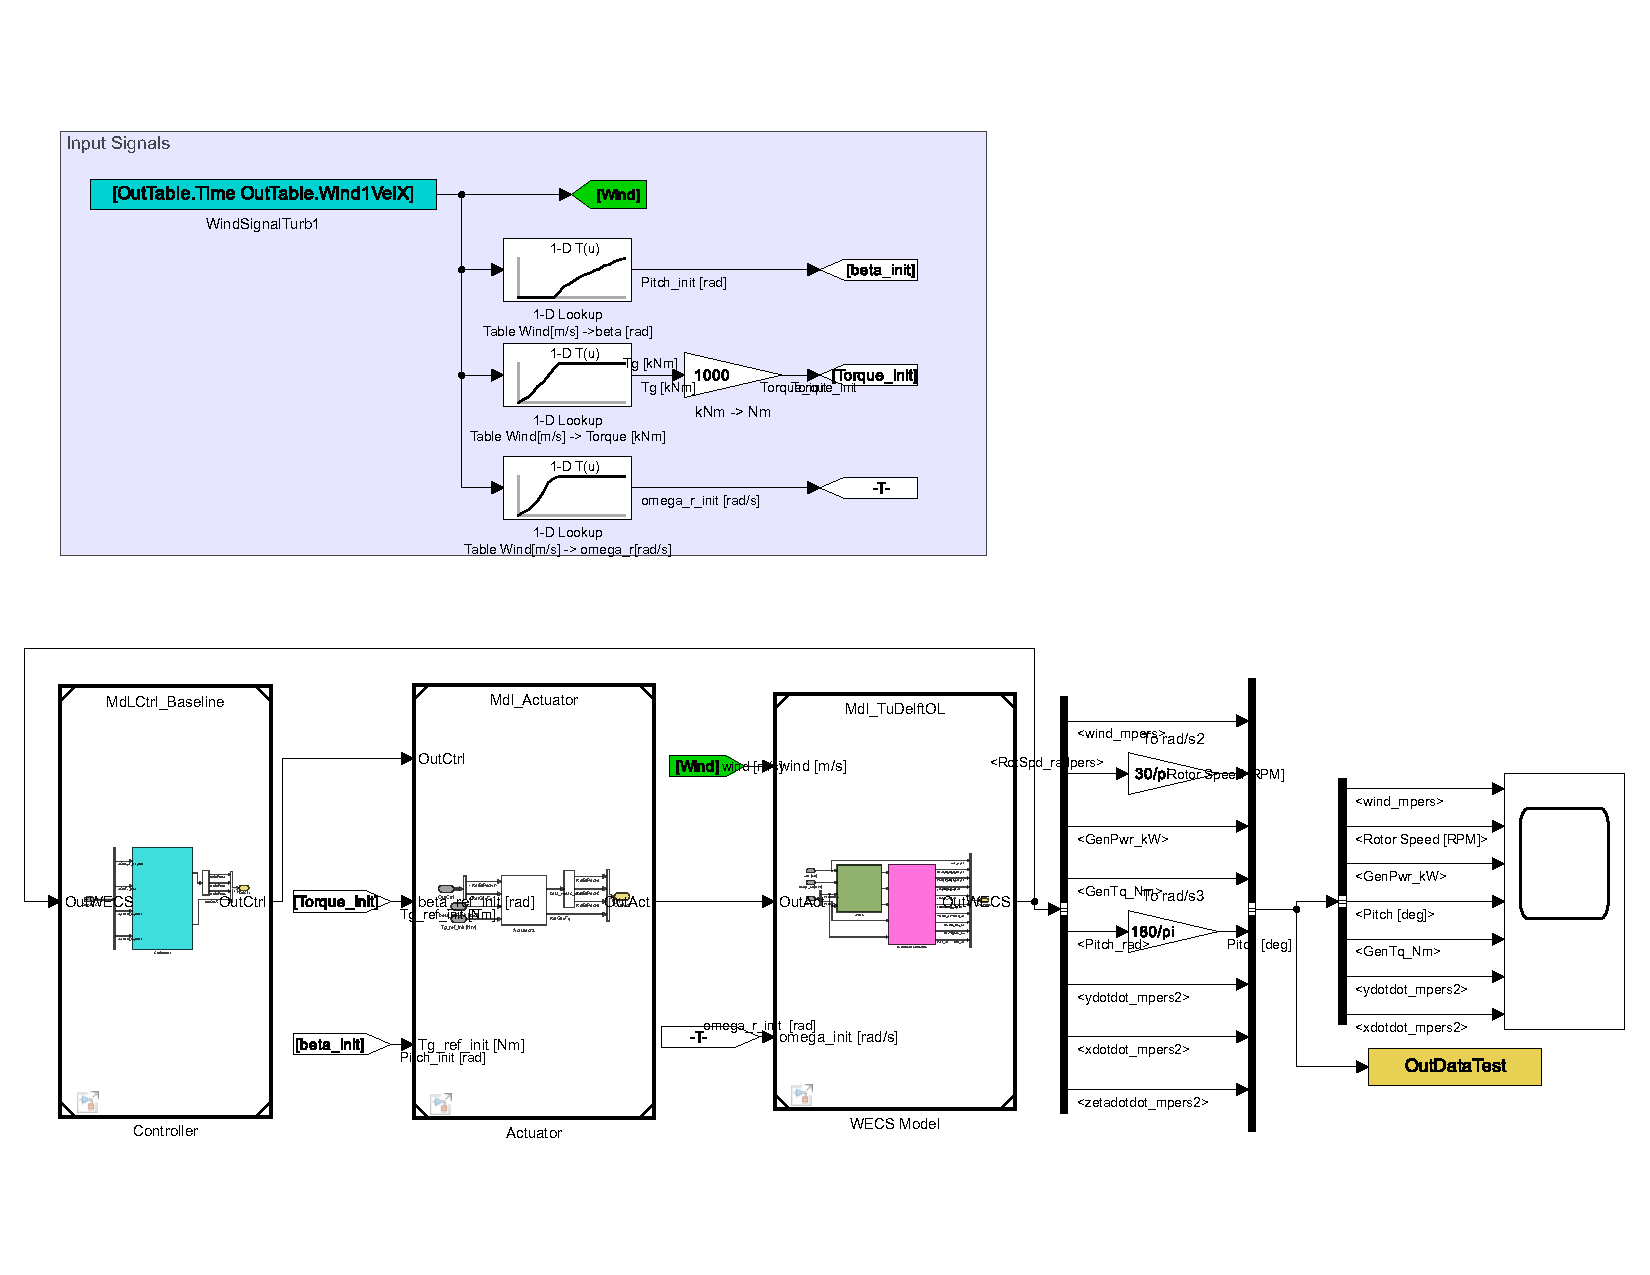
\includegraphics[width=0.9\textwidth, trim={0.2cm 2cm 0.2cm 2.cm}, clip]{figures/figures_Simulink/test_SimulinkMdl1_Baseline.pdf}
    \caption[Simulink model for closed loop verification including controller, actuator, and WECS model.]{Simulink model for closed loop verification including controller, actuator, and WECS model. The wind is created with the FASTTool and used for the initialization of the generator torque, the blade pitch and the rotor speed.}
   \label{fig:baseline_simulink}
\end{figure}
The baseline controller relies solely on generator speed feedback \(\omega_g\) and operates based on different control strategies across the turbine's operational regions. In Regions I 1/2 and II, the generator torque is determined using a \(k\omega^2\) control law, derived from a tabulated function of \(\omega_g\), maximizing power yield below rated wind speed. In Region III, a gain-scheduled PI controller modulates the collective blade pitch angle \(\beta_0\) to regulate power output. The proportional and integral gains, \(K_P(\omega_g)\) and \(K_I(\omega_g)\), are dynamically scheduled to track and maintain the rated rotor speed.
%
To prevent excitation of structural resonances, the FASTTool controller includes filters on the generator speed signal, such as a low-pass filter and two notch filters. The pitch control signal \(\beta_{\text{ref}}\) is determined based on the filtered generator speed \(\omega_{g,\text{filt}}\), ensuring stable power regulation above rated wind speed while mitigating structural loads. The controller allows for user selection between constant and gain-scheduled PI coefficients, with the latter used as the default setting, as detailed in \cite{mulders2020wind}.

The wind turbine model included in the Simulink implementation for closed loop testing is either the 5th or the 9th-order model described in Section~\ref{subsec:Structural Models}. Figure \ref{fig:ol_wecs_models} shows both models.
    
\begin{figure}[htbp]
    \centering
    \subfloat[5th-order model with rotor speed and tower displacement states, adapted from \cite{mulders2020preventing}.\label{fig:tudelft_ol_wecs}]{%
        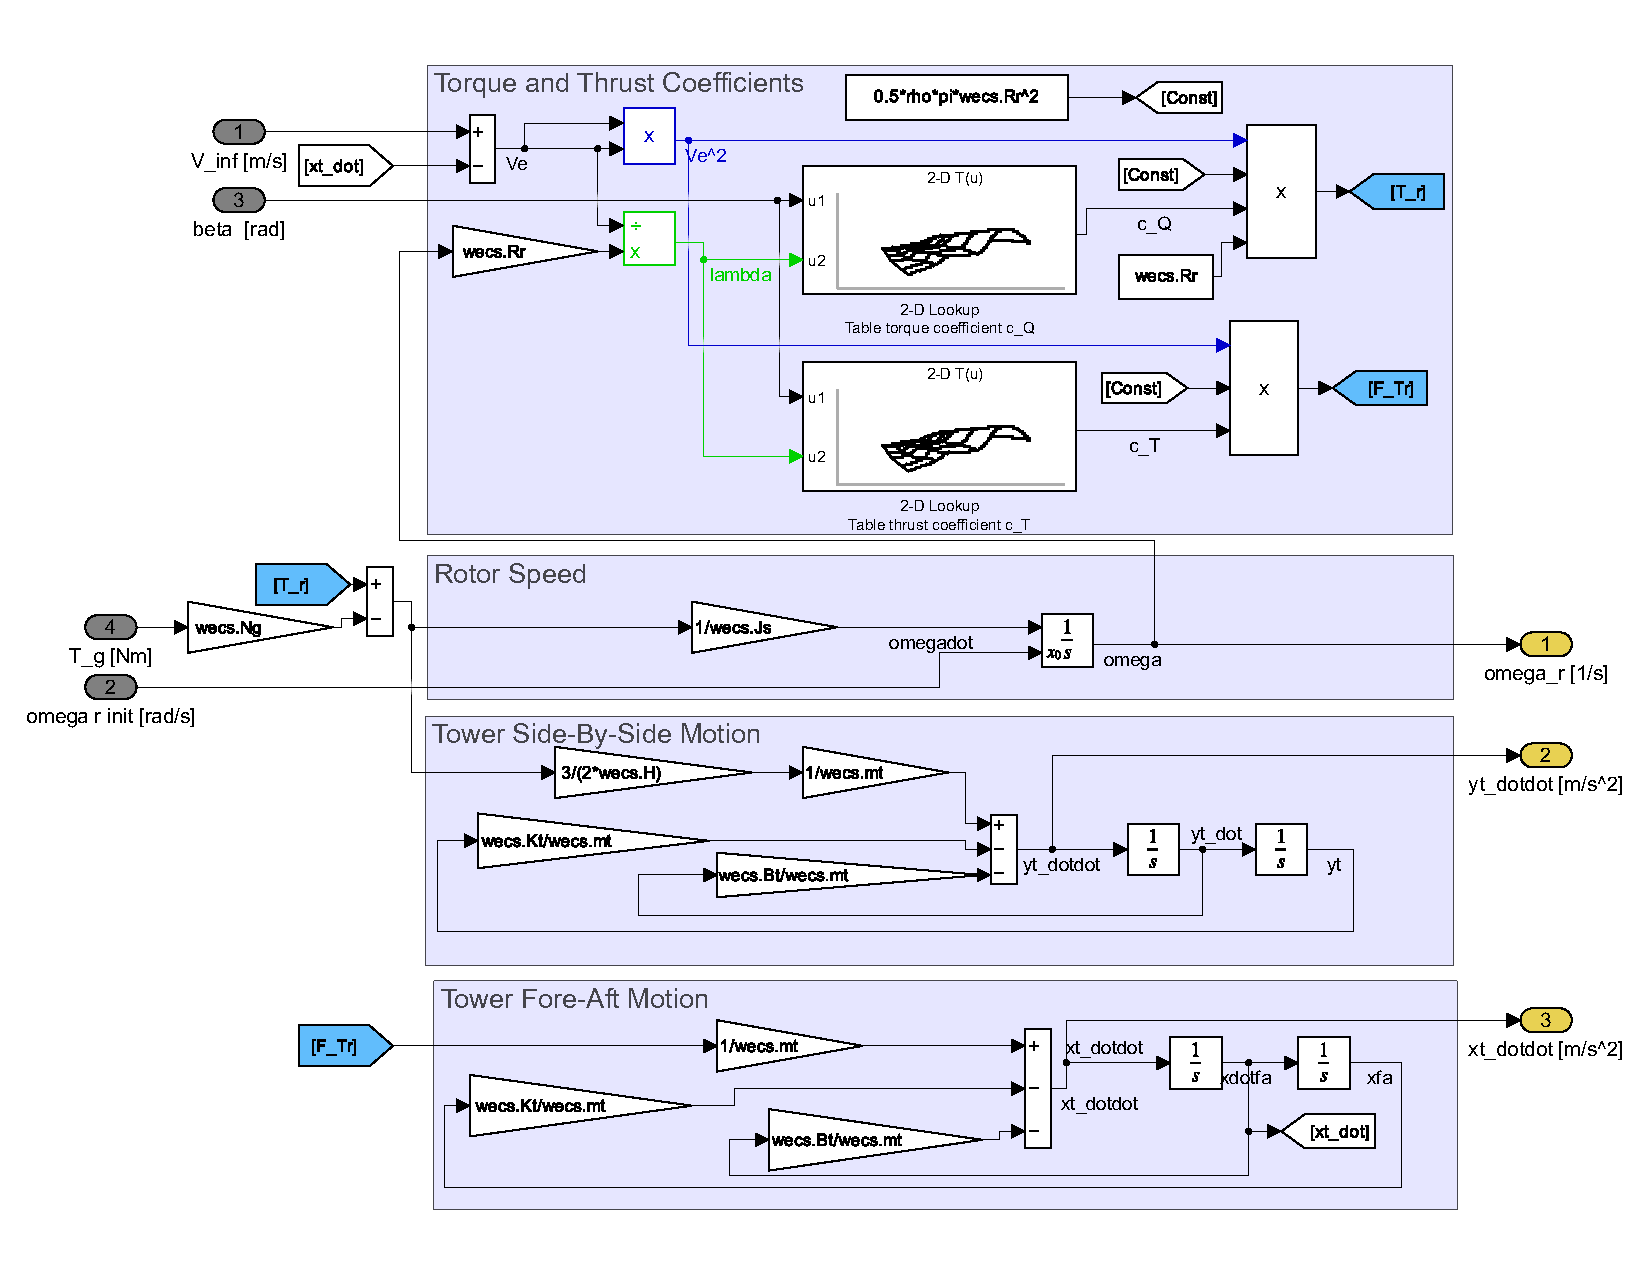
\includegraphics[width=0.9\textwidth, trim={0.2cm 0.5cm 0.2cm 1.cm}, clip]{figures/figures_Simulink/Mdl_TuDelftOL_WECS.pdf}
    }\\[1em]
    \subfloat[9th-order model with rotor and generator speed as well as tower and blade displacement states, adapted from \cite{Bianchi2007}.\label{fig:bianchi_ol_wecs}]{%
        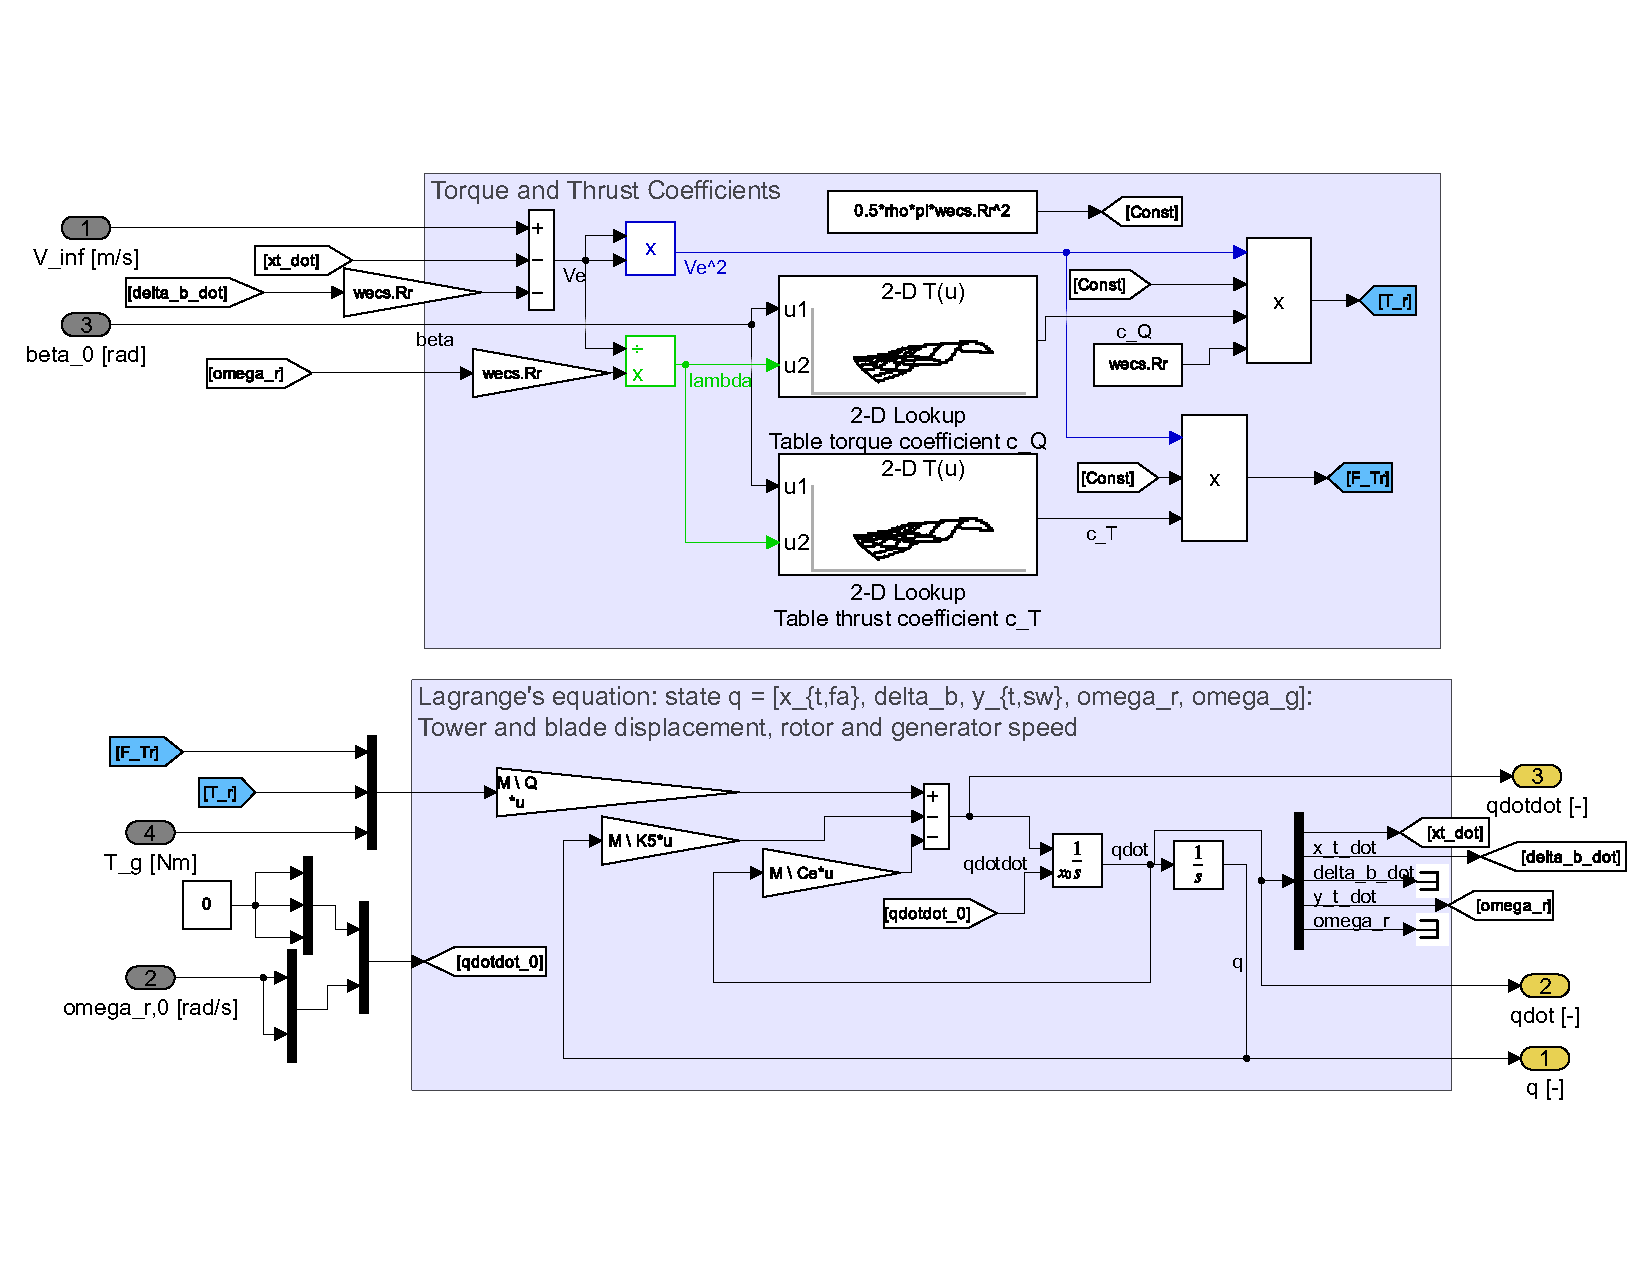
\includegraphics[width=0.9\textwidth, trim={0.1cm 2cm 0.2cm 2.8cm}, clip]{figures/figures_Simulink/Mdl_BianchiOL_WECS.pdf}
    }
    \caption[Simulink implementations of the two qLPV WECS models.]{Simulink implementations of the two qLPV WECS models. Both models use 2D lookup tables for the torque and thrust coefficient $c_T$ and $c_Q$, and have as inputs wind speed $V_\infty$, blade pitch angle $\beta$, and generator torque $T_g$.}
    \label{fig:ol_wecs_models}
\end{figure}

FASTTool is a MATLAB-based GUI used for configuring simulations and tuning controller parameters. It uses the FORTRAN-based FAST NREL 5MW wind turbine model implementation and integrates it into Simulink as an S-function. The baseline power controller is implemented using Simulink blocks and MATLAB functions. This controller is used to control both wind turbine models introduced above, as well as the Simulink S-function implementation of the FAST model. In the MIMO controller architecture presented in the next chapter, both the pitch and generator torque controllers of the baseline controller are replaced by the qLMPC scheme. For model verification purposes, however, the original Simulink implementation of the baseline controller is retained. The nonlinear differential equations of the two qLMPC models are implemented in Simulink. To verify the models, two simulations are performed using the original setup, including the baseline controller and the FAST NREL 5MW model implemented as an S-function. The first simulation consists of a wind-speed sweep from 4\,m/s to 25\,m/s in increments of 1\,m/s. Each wind-speed level is maintained for 100\,s to ensure that steady-state conditions are reached. This test is used to verify that the models converge to the same steady-state operating points and to compare their transient responses to wind-speed changes. The second simulation uses a turbulent wind field with a mean wind speed of 18\,m/s and IEC turbulence class B, corresponding to a turbulence intensity of 14\,\%. This simulation is used to investigate the qLPV models' responses to turbulent wind conditions. The first simulation is run for 2200\,s and the second for 660\,s. Both simulations are executed with a sampling time of 8\,ms, and the generated wind data are stored. Using these recorded wind speed time series, the simulations are repeated with the FAST NREL 5MW S-function replaced by the Simulink implementations of the qLPV models.

\newpage
\subsection{Results}\label{subsec:ResultsqLPVModel}
This section presents the open-loop frequency domain and closed-loop time domain verification of the two qLPV models.
\subsubsection*{Results Open-loop Frequency Domain Verification}
Figures~\ref{fig:Bode4} and~\ref{fig:Bode12} depict the magnitude response of four linear models: two models at the vertex wind speeds of 4\,m/s and 25\,m/s, and two models near the rated wind speed of 11.4\,m/s (specifically at 11\,m/s and 12\,m/s). Corresponding linearized FAST models serve as the reference.
\begin{figure} [htp]\center
 
    \subfloat[Wind speed $V_{\infty} = 4$\,m/s]{\includegraphics[width=0.75\textwidth]{Figures_ADi/BodeV4.eps}}\\
    \subfloat[Wind speed $V_{\infty} = 11$\,m/s]{\includegraphics[width=0.75\textwidth]{Figures_ADi/BodeV11.eps}}
   % \subfloat[Wind speed $V_{\infty} = 12$\,m/s]{\includegraphics[width=0.75\textwidth]{Figures_ADi/BodeV12.eps}}\\ 
  %  \subfloat[Wind speed $V_{\infty} = 25$\,m/s]{\includegraphics[width=0.75\textwidth]{Figures_ADi/BodeV25.eps}}
    \caption[Open-loop verification: Frequency response magnitude of linearized FAST and qLPV models for below rated wind speeds.]{Open-loop verification: Frequency response magnitude of linearized FAST and qLPV models for below rated wind speeds. Mdl1 (black dashed line), Mdl2 (blue line), and FAST reference implementation (red line) at frequencies from 0.01\,Hz to 2\,Hz.} %
    \label{fig:Bode4}
\end{figure}
\begin{figure} [htp]\center
    \subfloat[Wind speed $V_{\infty} = 12$\,m/s]{\includegraphics[width=0.75\textwidth]{Figures_ADi/BodeV12.eps}}\\ 
\subfloat[Wind speed $V_{\infty} = 25$\,m/s]{\includegraphics[width=0.75\textwidth]{Figures_ADi/BodeV25.eps}}
\caption[Open-loop verification: Frequency response magnitude of linearized FAST and qLPV models for above rated wind speeds.]{Open-loop verification: Frequency response magnitude of linearized FAST and qLPV models for above rated wind speeds. Mdl1 (black dashed line), Mdl2 (blue line), and FAST reference implementation (red line) at frequencies from 0.01\,Hz to 2\,Hz.} 
\label{fig:Bode12}
\end{figure}

 For all models, the frequency range from 0.01\,Hz to 2\,Hz is evaluated. Note that typically only the range up to 1\,Hz is considered in the literature, e.g., \cite{schlipf2013nonlinear} or \cite{pamososuryo2022individual}, as this interval contains the dominant first tower and blade modes. The magnitude response of the first (5th-order) model is shown in black, the second (9th-order) model in blue, and the linearized FAST reference in red. The latter's 30 states include all states of the derived qLPV models alongside additional structural degrees of freedom. The plots visualize the transfer functions from the control inputs (generator torque and blade pitch) and the disturbance (wind speed) to the rotor speed and tower fore-aft and side-to-side acceleration.
 
The comparison shows a good fit to the linearized FAST reference for both models from 0.01\,Hz up to the natural tower frequency at 0.3\,Hz. The second model also demonstrates a reasonable fit at the first blade natural frequency around 0.7\,Hz. However, the frequency behavior at higher frequencies exceeding 1\,Hz deviates from the FAST model. This deviation is due to higher-order dynamics present in the 30th-order linearized FAST model that are not captured in these simpler models. Thus, while the overall fit is reasonable, some discrepancy with the higher-order linearized FAST model is inevitable across different channels.

In the first column, the frequency response from the generator torque input is shown. From 0.01\,Hz up to approximately 0.7\,Hz, both reduced-order models follow the FAST reference closely. At lower wind speeds, depicted in Figure~\ref{fig:Bode4} as well as in Figure~\ref{fig:Bode12}(a), this is true for all three depicted output axes, i.e., the rotor speed, the tower fore-aft and side-to-side acceleration. At the highest wind speed, see Figure~\ref{fig:Bode12}(b), both models show a small deviation in the side-to-side acceleration at low frequencies that gradually closes as the tower frequency peak is approached. The side-to-side peak's frequency is captured accurately, though its magnitude is slightly underestimated. Above 1\,Hz, an additional resonance in the FAST reference, likely a blade mode, is not captured by either reduced-order model.

The second column shows the response to the blade pitch input. Blade pitch is not used for active control below rated wind speed, as in Figure~\ref{fig:Bode4}, and remains near a fixed angle. The pitch-to-output response therefore reflects the underlying open-loop aeroelastic dynamics, in which blade structural modes play a dominant role. As a result, differences between the reduced-order models become more apparent in this channel. Looking at the response of the rotor speed to the blade pitch, the agreement between the FAST reference and the 9th-order model is considerably better than with the 5th-order model. The advantage of the model with blade dynamics is also clear in the tower fore-aft acceleration response, where it reproduces the blade frequency peak around 0.7\,Hz, especially at 4\,m/s in Figure~\ref{fig:Bode4}a. At higher wind speeds, see Figure~\ref{fig:Bode12}, this peak is less pronounced, and differences among models diminish. Still, the 9th-order model, which includes blade dynamics, consistently provides a better overall fit across the full frequency range for the responses of the rotor speed and tower fore-aft acceleration. Interestingly, in the tower side-to-side acceleration response, the model without blade dynamics outperforms the one including them, particularly at low frequencies. This is likely because the blade mode in the 9th-order model is tuned to match fore-aft motion, which dominates the tower bending, whereas side-to-side effects require more detailed blade modeling than currently included.

The third column depicts the response to variations in wind speed. In the rotor speed response, a sharp notch appears in the FAST reference at approximately 0.34\,Hz, the frequency of the first tower mode, across all wind speeds. Both qLPV models reproduce this notch closely. At higher frequencies, however, Mdl1 continues along a smooth, monotonic decline, while Mdl2 dips more sharply at 0.7\,Hz before recovering to follow the slope of Mdl1. FAST does not dip at 0.7\,Hz, but at 0.8\,Hz for the two lower and around 1\,Hz for the higher wind speeds, still the amplitude of Mdl2 is closer to this reference than the one of Mdl1.

In the tower fore-aft acceleration response, both models again match FAST well through the tower peak at 0.34\,Hz. Past the peak, Mdl2 continues to track the FAST reference's mild increase at 0.7\,Hz, whereas Mdl1 diverges gradually as its response flattens. In both of these channels, Mdl2 therefore clearly outperforms Mdl1 at higher frequencies. In the tower side-to-side response, by contrast, Mdl1 and Mdl2 remain close to one another throughout the frequency range, but both substantially overestimate the FAST reference at low frequencies, with the gap closing as all three converge near the shared tower peak at 0.34\,Hz. Above this peak, the FAST reference drops, with this amplitude decrease not reproduced by either qLPV model. Instead, Mdl2 exhibit a secondary dip near 0.7\,Hz that is largely absent from the FAST reference, while Mdl1 shows a relative flat response. However, despite the comparatively weaker open-loop fit in the side-to-side channel, it will be discussed in the next section that this discrepancy has little practical impact. To verify that the reduced-order models accurately capture the dynamics within the frequency range relevant for control, a time-domain comparison with the FAST reference is also carried out in closed-loop operation. 


\subsubsection*{Results Closed-loop Time Domain Verification}    
For the verification in closed loop, two representative wind scenarios are considered: a stepped wind speed sweep from 4\,m/s to 25\,m/s, and a turbulent wind input with a mean speed of 18\,m/s.

Figure~\ref{fig:TimeCmpMdlSweep}(a) shows the results for the stepped wind sweep across all three closed-loop models. The wind increases in steps of 1\,m/s every 100\,s. The first 60\,s of the simulation, which contain initialization artifacts, are omitted. As a result, 40\,s of excitation is shown for 4\,m/s, and 100\,s for all other wind speeds. Figure~\ref{fig:TimeCmpMdlSweep}(b) presents the signals between 600\,s and 1000\,s of simulation time, corresponding to wind speeds between 10\,m/s and 13\,m/s. As before, the signals of the 5th-order model are plotted in black (dashed), the 9th-order model in blue, and the FAST model in red.
\begin{figure}[h]
    \centering
    \subfloat[Stepped wind sweep from 4\,m/s to 25\,m/s]{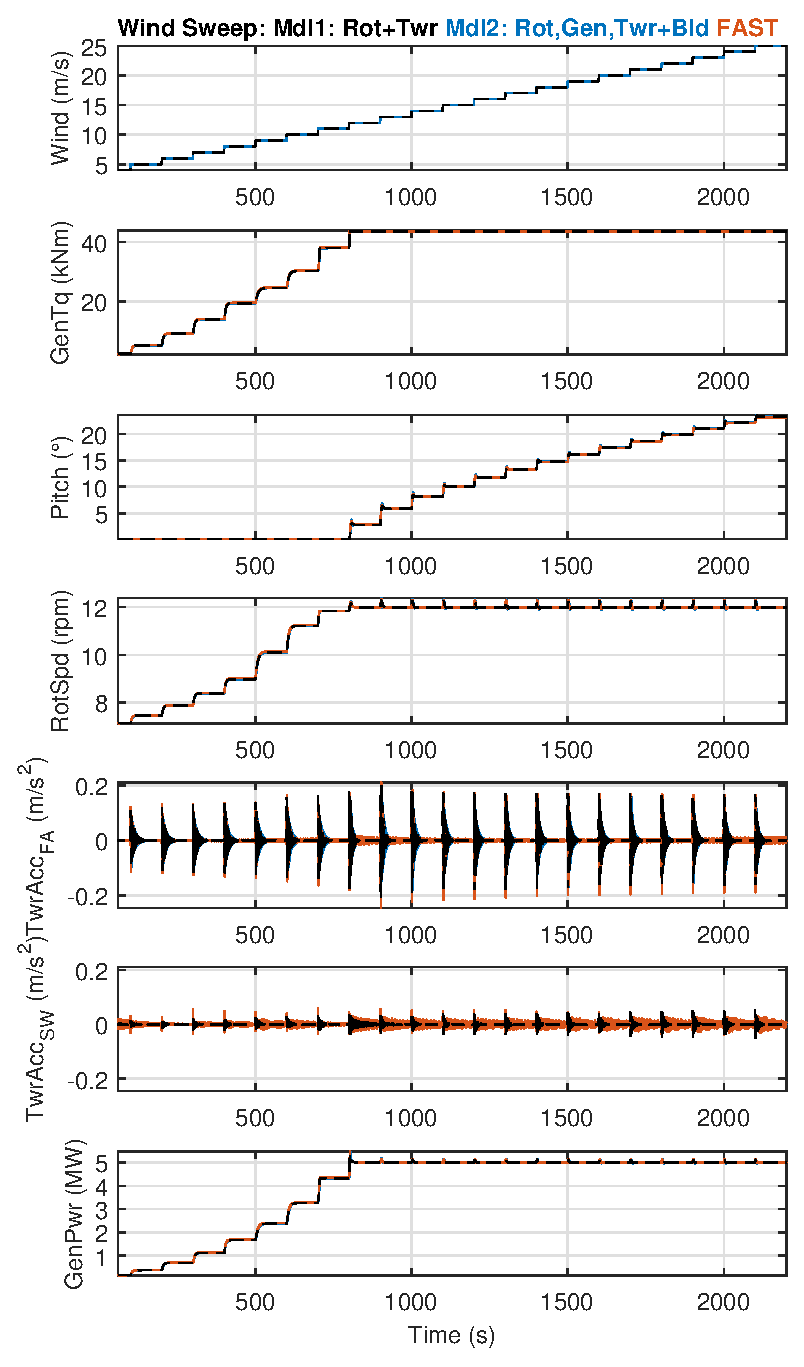
\includegraphics[width=0.435\textwidth]{figures/Figures_ADi/cmpTimeDomain_All.eps}}\hspace{0.01\textwidth}
    \subfloat[Zoom on wind speed range 10\,m/s to 13\,m/s]{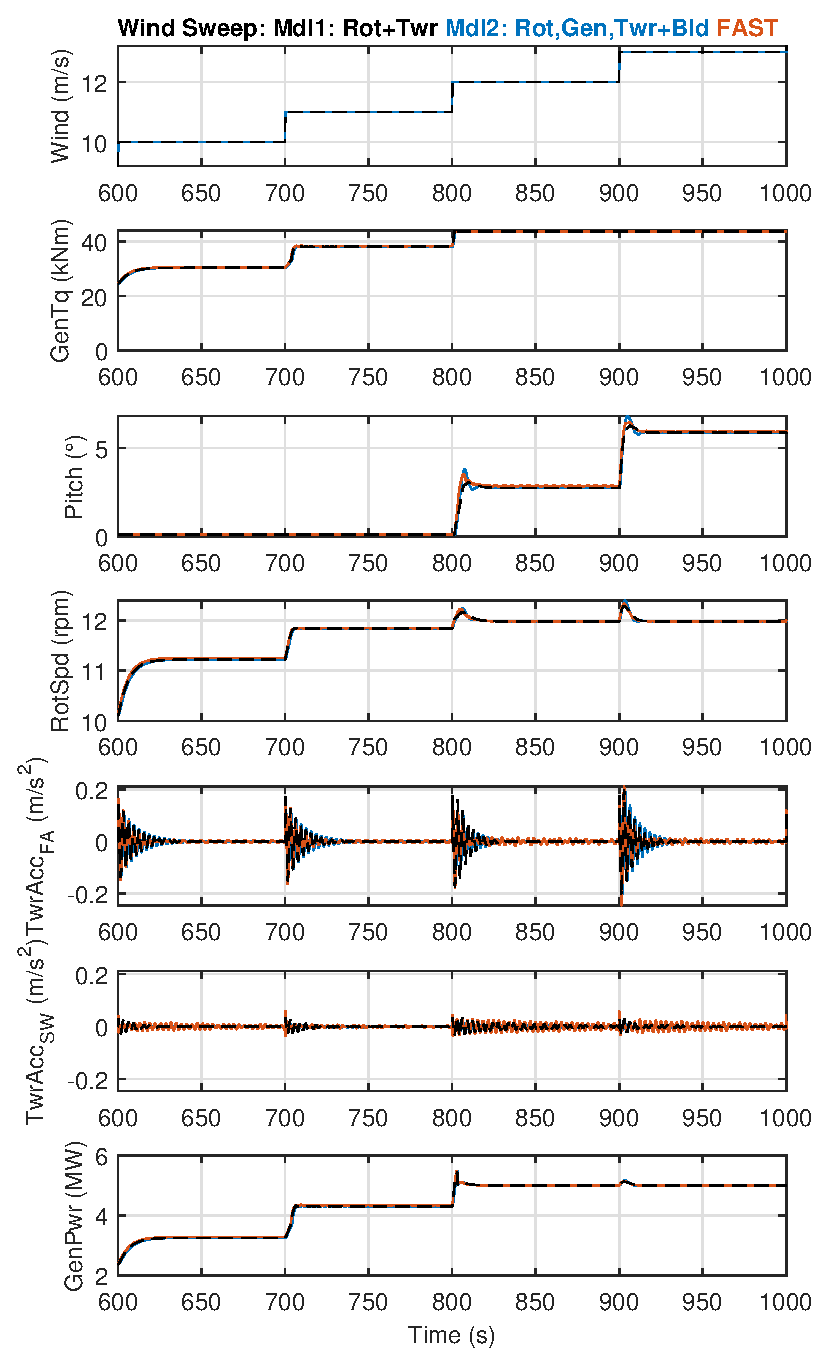
\includegraphics[width=0.45\textwidth]{figures/Figures_ADi/cmpTimeDomain_AllZoom.eps}}
    \caption[Closed-loop verification: FAST and qLPV models with PI baseline 
   controller, stepped wind sweep 4\,m/s to 25\,m/s.]%
   {Closed-loop verification: FAST and qLPV models simulated in closed loop with the PI baseline controller with a stepped wind sweep from 4\,m/s to 25\,m/s. 
       Mdl1 (black dashed line), Mdl2 (blue line), and FAST reference implementation (red line). Displayed signals: wind, control inputs, 
       rotor speed, tower accelerations, and power.}
    \label{fig:TimeCmpMdlSweep}
\end{figure}
%
The first subplot shows the wind input applied to the turbine, which is identical for all simulations. The second and third subplots display the two control inputs: generator torque and collective blade pitch. The fourth subplot shows the rotor speed, followed by the fifth and sixth subplots showing the tower fore-aft and side-to-side accelerations, respectively. The final subplot depicts the resulting electrical power output. There is an excellent fit between FAST and both models for the stepped wind sweep test case, in the transient dynamic as well as in the steady state gain. The good fit in steady state corresponds to the resemblance between FAST and both models for the rotor speed and the tower fore-aft acceleration for lower frequencies. As there is little difference both in the generator torque as well as in the rotor speed, there is also a good fit in the power output. There is also a good fit in the amplitude of the fore-aft tower acceleration for all wind speeds. The only signal that is not matched well is the tower side-to-side acceleration. However, the amplitudes of this signal is comparably small and its influence on the overall dynamics is nearly negligible.

Figure~\ref{fig:TimeCmpMdlNTM} shows the second test case: a turbulent wind profile with a mean speed of 18\,m/s and IEC turbulence class B. This test case reveals a limitation of the qLPV models, which represent wind as a scalar value acting uniformly on the rotor, rather than as a spatially distributed field.
\begin{figure}[h]
    \centering
    \subfloat[No filter]{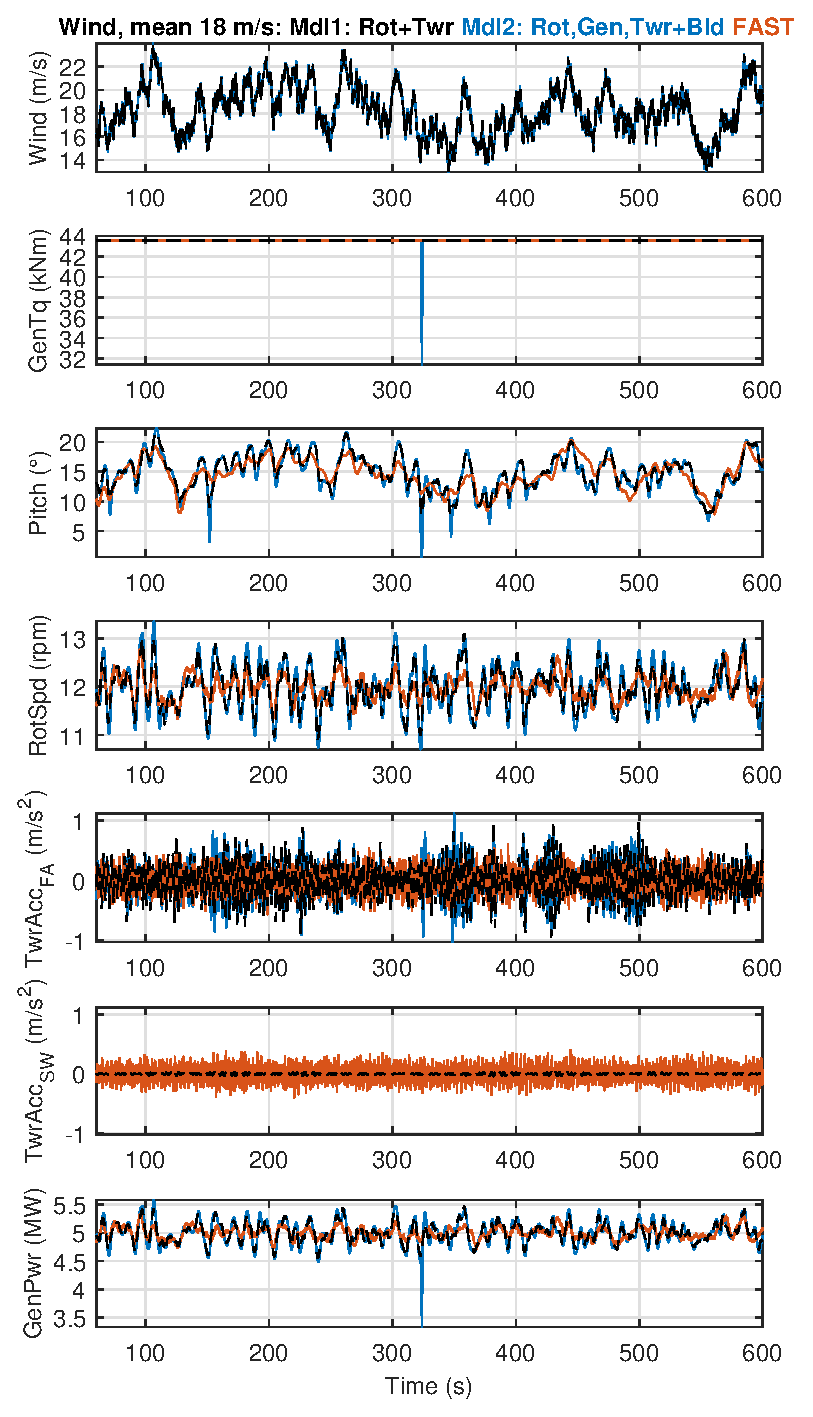
\includegraphics[width=0.45\textwidth]{figures/Figures_ADi/cmpTimeDomain_AllNTW18.eps}}\hspace{0.01\textwidth}
    \subfloat[Filter with $k_\tau = 0.75$ and  $k_T = 0.25$ ]{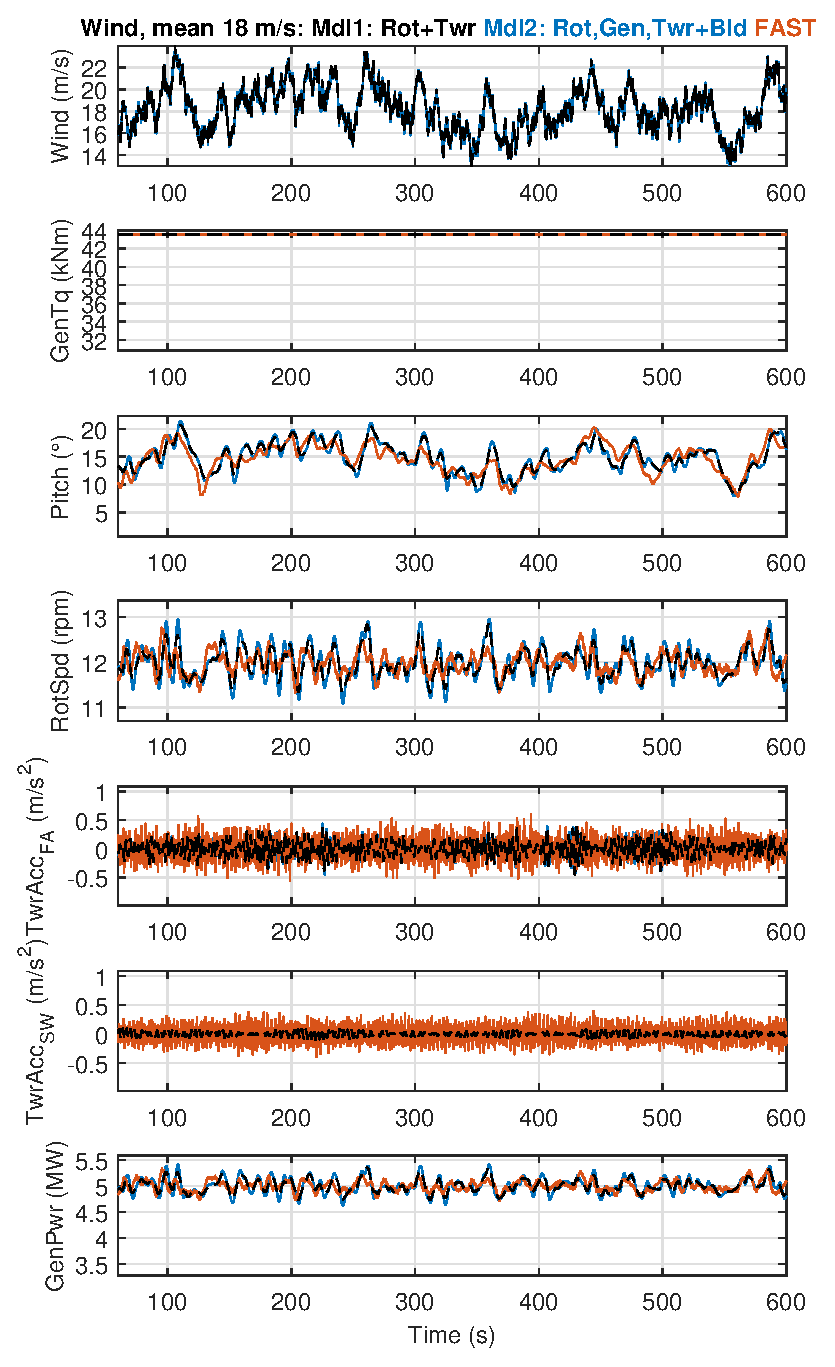
\includegraphics[width=0.45\textwidth]{figures/Figures_ADi/cmpTimeDomain_AllNTW18_kVe0dot25_kVeTau0dot75.eps}}
    \caption[Closed-loop model comparison: FAST and qLPV models with baseline 
    PI controller, under turbulent wind with and without filter on freestream wind.]{Closed-loop model comparison: FAST and qLPV models with PI baseline controller, under turbulent wind, 18\,m/s mean, IEC turbulence 
        class B (14\,\%), with and without filter on freestream wind. Mdl1 (black 
        dashed line), Mdl2 (blue line), and FAST reference implementation (red 
        line). Displayed signals: wind, control inputs, rotor speed, tower 
        accelerations, and power.}
    \label{fig:TimeCmpMdlNTM}
\end{figure}
In a real turbine, the large rotor disk acts as a natural low-pass spatial 
filter, averaging out high-frequency point gusts across its swept area. 
Because single-point freestream wind files lack this spatial coherence, 
feeding an unfiltered point velocity into the low-order lookup tables causes 
the model to respond excessively to high-frequency variations. At the same 
time, structural tower dynamics are driven by localized aerodynamic thrust 
forces and blade-passage effects, which require a faster excitation spectrum. 
To address this discrepancy, a velocity-dependent low-pass filter is applied 
to the freestream wind input, with separate scaling factors for the torque 
($k_\tau = 0.75$) and thrust ($k_T = 0.25$) channels to preserve the 
relevant excitation frequencies for each. As shown in Figure~\ref{fig:TimeCmpMdlNTM}(a), without filtering the models 
exhibit pronounced high-frequency oscillations and overshoot in blade pitch, 
rotor speed, and generator power. With the filter active in Figure~\ref{fig:TimeCmpMdlNTM}(b), the amplitudes more 
closely follow the FAST reference while the tower fore-aft acceleration 
retains sufficient high-frequency excitation. Note that these filters are used 
only for the turbulent wind comparison with FAST and are not included in the 
qLMPC controller design, where the freestream wind speed $V_\infty$ is used 
directly as an input.

It should also be noted that some minor discrepancies remain in Figure~\ref{fig:TimeCmpMdlSweep}, such as small oscillations in the tower movement due to FAST's full degrees of freedom. However, the reduced-order models capture the dominant system dynamics with sufficient accuracy for control design. Both Mdl1, without blade dynamics, and Mdl2, with an additional blade flapwise degree of freedom, show good agreement with the FAST reference during the stepped wind sweep. Mdl2 captures a broader range of dynamics, most notably in the blade pitch to rotor speed channel, where it shows better alignment with FAST due to the inclusion of blade dynamics. Furthermore, Mdl2 enables the representation of blade out-of-plane moments, which is relevant for evaluating damage equivalent loads used as one of the performance criteria for controller evaluation. Therefore, Mdl2 is selected as the basis for the qLMPC design.

